\chapter[Solução Eletrônica]{Solução Eletrônica}

Este capítulo é voltado para o desenvolvimento do sistema eletrônico, apresentando as escolhas de projeto a partir dos requisitos técnicos. Assim, a solução de eletrônica será dividida em 3 sistemas: Módulo de Medição, Central de Controle e Acionamento de Atuadores. Consequentemente, os 3 sistemas possuem grande dependência entre si.

\section{Módulo de Medição}

O módulo de medição é o sistema que tem a  funcionalidade de realizar a captura de dados de interesse para uso no controle e na automação do dispositivo. Sendo assim, trata-se de um sistema micro-controlado pela central de controle conectado a vários componentes de detecção e medição. Dessa forma, os componentes de detecção e medição foram selecionados a partir dos requisitos levantados, disponibilidade no Brasil, apresentarem custos acessíveis e escala de medição compatível com a aplicação.

% \begin{itemize}
    % \item Sensor de Temperatura e Umidade
    \subparagraph*{$\bullet$ Sensor de Temperatura e Umidade} \hfill
    
    O uso do sensor de temperatura e de umidade foi baseado na necessidade do monitoramento constante das variáveis de temperatura e umidade relativa dentro do dispositivo. A maioria dos medicamentos sólidos precisa estar armazenada em uma faixa de temperatura e umidade relativa determinada pelo fabricante para não alterar as propriedades químicas e a eficácia deles. 
    
    Para seleção do componente foram priorizados sensores com mais de uma funcionalidade, logo, sensores de temperatura e umidade relativa integrados. Sendo assim, a faixa de valores para a conservação de medicamentos sólidos está entre 15 $^\circ$C e 30 $^\circ$C e a escala de umidade relativa de 40\% a 70\% \cite{Pinto_2016}. Adicionalmente, deve ser levado em consideração, para escolha de um sensor em determinada aplicação, os parâmetros de acurácia, precisão, sensibilidade e resolução \cite{webster2018measurement}. 
    
    Como os parâmetros medidos de temperatura e umidade, não são unidades de mudança rápida em pequenos intervalos de tempo (menor 1 segundo) no ambiente em que ele está inserido, o sensor escolhido não precisa ter uma taxa de atualização maior que 1 Hz \cite{webster2018measurement}. Mas é preferível escolher aqueles com maior resolução, funcionar na faixa de conservação do medicamento e uma precisão menor que 1 $^\circ$C para temperatura e 5\% UR para umidade relativa para diminuir a faixa de dúvida do sensor utilizado. Por fim deve ser priorizado os sensores em um módulo comercial que entrega os dados de forma digital em um protocolo compatível com a central de controle da solução eletrônica. Ou seja, saída compatível com os protocolos \textit{Inter-Integrated Circuit} (I$^2$C), \textit{Serial Peripheral Interface} (SPI), \textit{Universal asynchronous receiver/transmitter} (UART), \textit{Display Serial Interface} (DSI) ou \textit{Camera Serial Interface} (CSI).
    
    Sendo assim, o sensor selecionado foi o \textbf{HTU21D} embarcado em um módulo comercial. Devido a ser um sensor compatível com as faixa de captura, resolução e precisão dos dados, preço de compra menor que R\$ 50,00  e o sinal de saída digital no protocolo interface I$^2$C, compatível com a central de controle.
    
    Para este sensor, nenhum condicionamento é necessário para o sinal, por ser realizado internamente no módulo. A conexão do sensor com a central de controle consiste em 4 pinos: VDD/VCC, GND e duas linhas de dados para comunicação I$^2$C (SDA/SCL). Além do mais, possui resolução configurável por \textit{software}, sendo 8/12 \textit{bits} para umidade e 12/14 bits para temperatura. O módulo \textbf{HTU21D} está representado na Fig. \ref{fig:sensor_temp_umidade}, e possui as seguintes especificações:

    \begin{itemize}
    \item[ ]
        \begin{itemize}
            \item Alimentação: 1,5 V a 3,6 V;
            \item Consumo de corrente em medição: 500 $\mu$A;
            \item Faixa de medição da umidade: 0-100\% UR;
            \item Faixa de temperatura de medição: -40 a 105 $^\circ$C;
            \item Precisão da umidade (10\% a 95\% UR):  $\pm$ 2\% UR;
            \item Precisão da temperatura: $\pm$ 0.3 $^\circ$C;
            \item Máximo consumo de energia ( Média de 8 bits de comunicação): 2,7 $\mu$W;
            \item Comunicação: I$^2$C;
            \item Dimensões: 15,8 x 15,6 x 2 mm;
            \item Preço: R\$ 18,90.
        \end{itemize}
    \end{itemize}
    
    \begin{figure}[H]
        \centering
        \subfloat[][Sensor HTU21D]{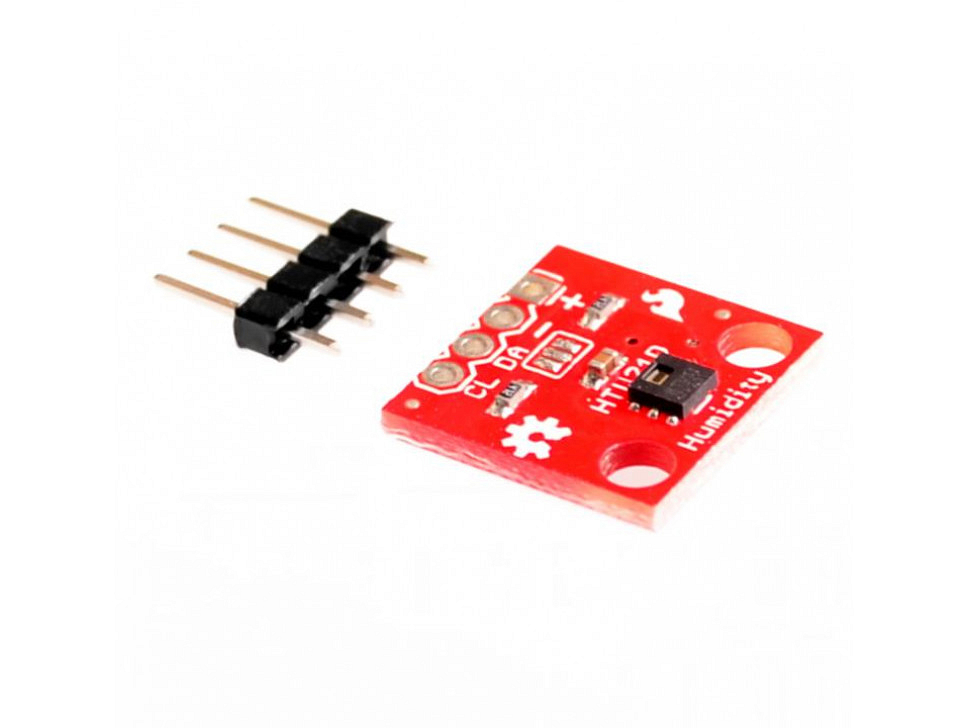
\includegraphics[width=0.3\textwidth]{figuras/eletronica/fotos_componentes/sensor_temp_umi.jpg}\label{fig:sensor_temp_umi_pic}}
        \hspace{0.1\textwidth}
        \subfloat[][Conexões do Sensor HTU21D]{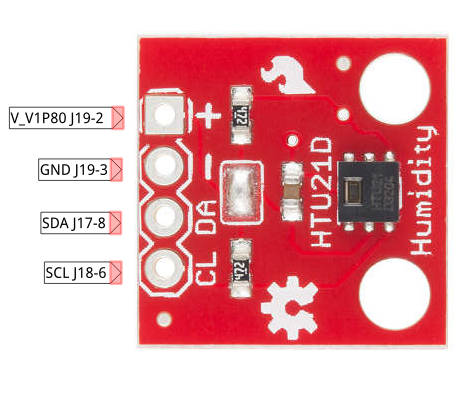
\includegraphics[width=0.2\textwidth]{figuras/eletronica/esquematicos/HTU21D.jpg}\label{fig:sensor_temp_umi_esq}}
        \caption{Sensor de Temperatura e Umidade}\label{fig:sensor_temp_umidade}
    \end{figure}
    
    
    
    % Atualizar nome de interruptor para chave
    \subparagraph*{$\bullet$ Chave} \hfill
    
    O uso de chaves se deve a necessidade de detectar o trancamento do compartimento frontal, por onde ocorre a passagem dos copos com medicamento do dispositivo, e do compartimento traseiro, por onde ocorre o acesso aos contêineres de estoque com medicamento. Da mesma forma, se é utilizada para detectar se os contêineres individuais, onde são colocados os medicamentos, foram encaixados corretamente.
    
    Com base na aplicação levantada foram selecionadas, de forma qualitativa, as chaves do tipo \textit{micro switch} \textbf{KW10-B} com haste. Uma vez que seu uso é ideal para as aplicações de detecção do trancamento de todas as portas do dispositivo e se os contêineres foram encaixados corretamente dados: a direção em que a chave é ativada; o mecanismo relacionado ao acoplamento e desacoplamento; a força mínima necessária para a ativação; a necessidade de um pequeno espaço de contato; possuir ação rápida; ter alta sensibilidade e; o pequeno deslocamento de operação.
    
    A chave tipo \textit{micro switch} \textbf{KW10-B} contêm 3 pinos de conexão: o terminal 1 - comum, o terminal 2 - normal aberto (em inglês \textit{normal open}) e o terminal 3 - normal fechado (em inglês \textit{normal closed}). Como o uso da chave se baseia em realizar uma alteração na conexão I/O com a central de controle quando ele é fechado a conexão entre a chave e a central de controle é feita usando os terminais 1 e 2, ou seja, comum e normal aberto. 
    
    
    A chave \textbf{KW10-B} está representada na Fig. \ref{fig:micro_switch_pic} e a lógica dos terminais podem ser visualizadas na representação esquemática da Fig. \ref{fig:micro_switch_esq}. O componente possui as seguintes especificações para a aplicação em que é utilizado:
    
   \begin{itemize}
    \item[ ]
        \begin{itemize}
            \item Alimentação: 5 V;
            \item Consumo de corrente máximo: 1 A;
            \item Quantidade de terminais: 3;
            \item Preço: R\$ 0,76.
        \end{itemize}
    \end{itemize}
    
    \begin{figure}[H]
        \centering
        \subfloat[][\textit{Micro Switch} KW10-B]{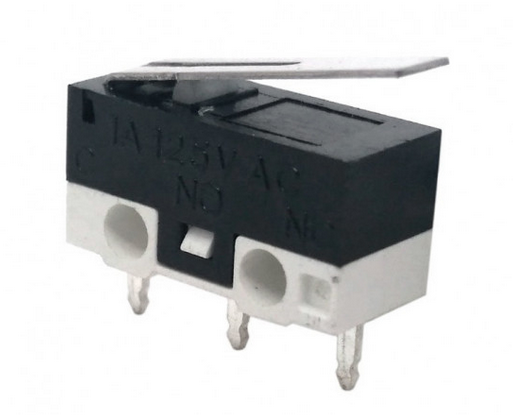
\includegraphics[width=0.2\textwidth]{figuras/eletronica/fotos_componentes/microswitch.png}\label{fig:micro_switch_pic}}
        \hspace{0.1\textwidth}
        \subfloat[][Conexões da Chave]{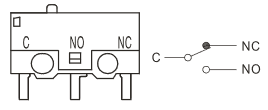
\includegraphics[width=0.3\textwidth]{figuras/eletronica/esquematicos/SW_1.png}\label{fig:micro_switch_esq}}
        \caption{Chave tipo \textit{Micro Switch}}\label{fig:micro_switch}
    \end{figure}
    
    % \item Sensor Fotoelétrico
    \subparagraph*{$\bullet$ Sensor Fotoelétrico} \hfill
    
    Os sensores fotoelétricos trabalham com emissão e recepção de luz e são ideais para aplicações onde faz-se necessário a detecção de objetos sem o contato físico. Dessa forma, estes sensores serão utilizados para detectar a passagem do medicamento sólido tanto na saída das comportas quanto no final da zona de transição. Além do mais, também será utilizado esse sensor para as seguintes detecções: presença do copo no reservatórios de copos, identificação da presença do copo em local predeterminado para o processamento de imagem, passagem do copo com medicamentos errados para o compartimento traseiro e passagem do copo para o compartimento frontal.
    
    Assim, optou-se pela utilização do sensor de barreira (foto interruptor), o qual o emissor e o receptor são instalados frente a frente para permitir que a luz do emissor entre no receptor. Logo, quando um objeto passa entre o emissor e o receptor a luz que entra no receptor é interrompida ou reduzida e assim é possível detectar a presença de um objeto, conforme as Fig. \ref{fig:sensor_infra} e  \cite{amron_photo_sensors}.
    
    \begin{figure}[H]
        \centering
        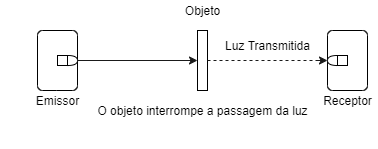
\includegraphics[width=0.5\textwidth]{figuras/eletronica/fotos_componentes/sensor_infra.png}
        \caption{Sensores de Barreira}
        \label{fig:sensor_infra}
    \end{figure}
    
    Por se tratar de um sensor de simples implementação, optou-se por fazer a implementação utilizando: um \textit{LED} emissor de infravermelho (\textbf{IR333C}), um fototransistor receptor de infravermelho (\textbf{PT333-3B}) e circuito comparador.
    
    Dessa forma, para construção do circuito do sensor fotoelétrico de barreira deve-se determinar a resistência de polarização do LED \textbf{IR333C} e determinar a potência do resistor conforme as Eq. \ref{eq:res_LED} e \ref{eq:Pot_Res}:
    
    \begin{equation}
        R_{LED} = \frac{(V_{Fonte} - V_{LED})}{I_{LED}} = \frac{( 5 - 1,5) \hspace{0.1cm} [\text{V}]}{20 \hspace{0.1cm} [\text{mA}]} = 175 \quad [\Omega]
        \label{eq:res_LED}
    \end{equation}
    
        \begin{equation}
        P_{R_{LED}} = V_{RES} \cdot I_{LED} = 3,5 \hspace{0.1cm}
        [\text{V}] \cdot 20 \hspace{0.1cm} [\text{mA}] = 0,07 \quad [\text{W}] 
        \label{eq:Pot_Res}
    \end{equation}
    
    Consequentemente, foi selecionado o resistor de 180 $\Omega$ por se tratar de um resistor comercial. A Fig. \ref{fig:esq_sensor_barreira} mostra o esquemático do circuito, enquanto a lista descreve os materiais a serem utilizados na construção.
    
    \begin{figure}[H]
    \centering
    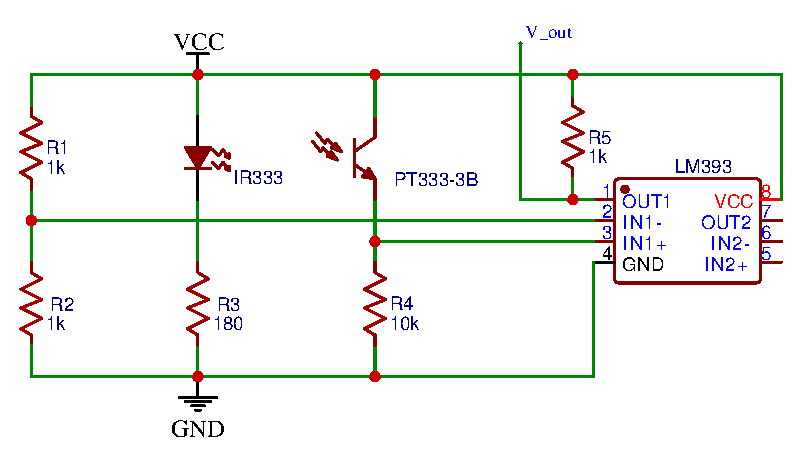
\includegraphics[scale=0.7]{figuras/eletronica/esquematicos/sensor_barreira/Schematic_Sensor_barreira.pdf}
    \caption{Esquemático do circuito do sensor fotoelétrico de barreira}
    \label{fig:esq_sensor_barreira}
    \end{figure}
    
    \begin{itemize}
    \item[ ]
        \begin{itemize}
            \item 1 LED IR333;
            \item 1 Fototransistor PT333-3B;
            \item 1 CI LM393;
            \item 1 Resistor de 180 $\Omega$;
            \item 1 Resistor de 10 k$\Omega$;
            \item 3 Resistores de 1 k$\Omega$.
        \end{itemize}
    \end{itemize}
    
    Para realizar as simulações foi utilizado o Opto-acoplador \textbf{4N25}, no qual consiste em um CI que contém um LED emissor de infravermelho e um fototransistor NPN. Optou-se pela utilização desse componente na simulação, uma vez que, os valores de tensão e corrente de entrada e saída são os mesmos para os componentes selecionados \textbf{IR333} e \textbf{PT333-3B}. Entretanto, a única variação do \textbf{4N25} em relação ao LED emissor \textbf{IR333} é a corrente de entrada de 50 mA para o circuito integrado (C.I.) e 20 mA para o LED, o que pode ser corrigido na simulação pela alteração do resistor do LED.
    
    %rever
    Outrossim, na simulação de acordo com a Fig. \ref{fig:sim_sensor_barreira}, foi adicionada uma sequência de pulsos na entrada do LED emissor para representar a passagem do objeto entre o emissor e o receptor. Uma vez que, com a passagem do objeto tem-se a ausência de luz, as junções inversamente polarizadas do fototransistor não conduzem corrente elétrica, e se tem como resultado uma resistência ``infinita''. Após a passagem do objeto, ocorrerá a entrada de luz nestas junções e sua resistência diminuirá, havendo assim a condução de corrente elétrica. 
    
    Decorrida essa variação de corrente, tem-se uma consequente alteração na tensão e dessa forma é possível utilizar o C.I. \textbf{LM393}, que contém dois amplificadores operacionais comparadores de tensão. Por conseguinte, liga-se a entrada inversora do comparador a um par de resistores cujos valores determinam a tensão de referência. Quando o valor na entrada não-inversora for maior que o valor de referência na entrada inversora a saída do comparador tende a 5 V. Enquanto que, quando o valor na entrada não-inversora for menor que o valor de referência na entrada inversora, a saída do comparador converge a 0 V. 
    
    \begin{figure}[H]
    \centering
    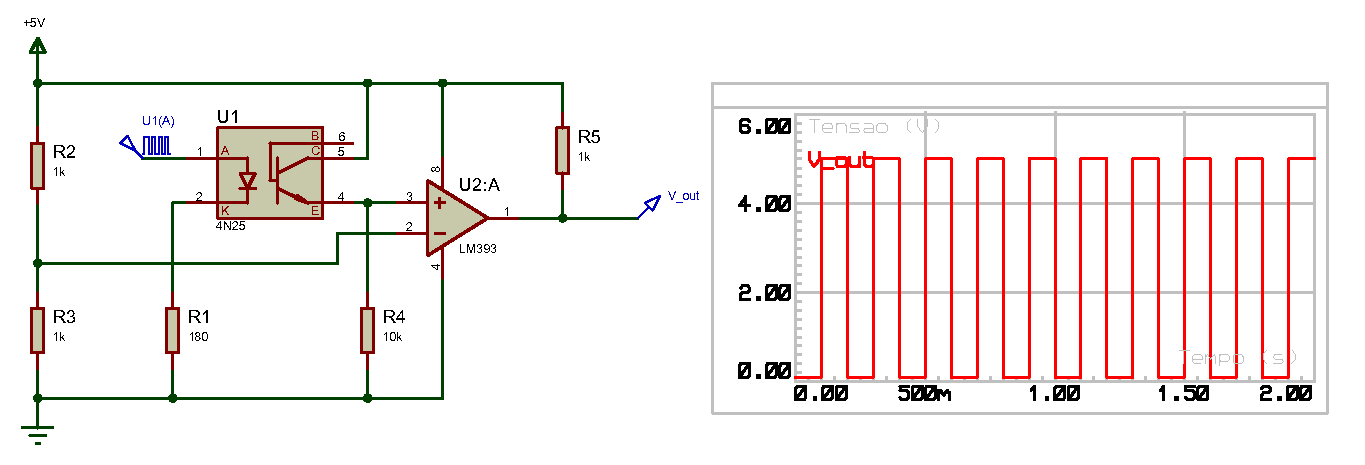
\includegraphics[scale=0.65]{figuras/eletronica/esquematicos/sensor_barreira/Sim_sensor_barreir_3.PDF}
    \caption{Simulação do Sensor Fotoelétrico de barreira}
    \label{fig:sim_sensor_barreira}
    \end{figure}
    
     Portanto, a partir dessa variação de tensão na saída pode-se detectar a passagem do objeto traduzindo a oscilação de 5 V e 0 V para uma representação digital ao ser conectado com a central de controle. Essa conexão utiliza 3 pinos: Terminal 1 é a alimentação do circuito em 5 V, Terminal 2 é o terra (em inglês \textit{Ground} - GND) e o Terminal 3 é a saída do comparador \textbf{LM393}, representado como $V_{out}$ na o esquemático da Fig. \ref{fig:sim_sensor_barreira}. Como a saída $V_{out}$ é uma saída digital, ou seja, quando for 0 V temos \textit{bit} 0 e em 5 V temos \textit{bit} 1, não é necessário o uso de um condicionamento de sinal como de conversores analógico-digital para conexão entre o sensor desenvolvido e a central de controle.

    Para levantamento da corrente total consumida pelo sensor de barreira é levada em consideração a corrente típica de operação para o \textit{LED} emissor ($I_{LED}$) e a corrente da fonte de alimentação para simulação na Fig. \ref{fig:sim_sensor_barreira} excluindo o IN25 ($I_{CIRCUITO}$). Como $I_{LED} =$ 20 mA e $I_{CIRCUITO} =$ 5 mA  obtemos a corrente total somando-as. Ou seja, $I_{total} = I_{LED} + I_{CIRCUITO} =$ 25 mA.  
    
    Por último, a partir da simulação foi realizada a placa de circuito impresso conforme a Fig. \ref{fig:PCB_barreira} no apêndice \ref{app:PCB}.  

    % \item Sensor de Biometria
    \subparagraph*{$\bullet$ Sensor de Biometria} \hfill
    
    O sensor de biometria é utilizado para autenticação de usuários nos mais diversos produtos no mercado. O seu funcionamento se baseia na captura da digital do usuário por meio de uma imagem que posteriormente terá suas características únicas extraídas e comparadas com um banco de dados de digitais cadastradas. 
    
    Dessa forma foi escolhido o sensor óptico de digitais \textbf{DY50}, Fig. \ref{fig:sensor_biometria}, por ser o mais comum no mercado e possuir um sistema  validado para obtenção de digitais. Esse sensor tem a funcionalidade de legitimar o funcionário da clínica geriátrica e permitir realizar funções que necessitam de autenticação. Assim, esse sensor é empregado para liberar o compartimento frontal/traseiro para a retirada da dose medicamentosa do dispensador e realizar o abastecimento do estoque de medicamentos.
    
   A conexão do sensor com a central de controle consiste em 4 pinos, e seu esquemático consta na Fig. \ref{fig:biometria_esq}: VCC e GND para alimentação, TX e RX para a comunicação UART. O sensor de biometria \textbf{DY50} está representado na Fig. \ref{fig:biometria_fig}, e possui as seguintes especificações:
    
    \begin{itemize}
    \item[ ]
        \begin{itemize}
            \item Alimentação: 3,6 V a 6 V;
            \item Consumo de corrente máximo: 120 $m$A;
            \item Taxa de transmissão : 9600, 19200, 28800, 38400, 57600 bits por segundo (bps);
            \item Comunicação: \textit{Transistor Transistor Logic} serial (TTL serial);
            \item Preço: R\$ 69,00.
        \end{itemize}
    \end{itemize} 
    
    \begin{figure}[H]
        \centering
        \subfloat[][Sensor DY50]{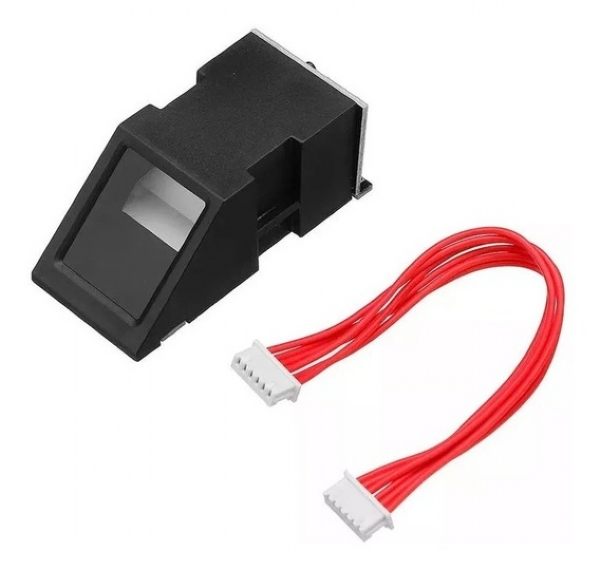
\includegraphics[width=0.3\textwidth]{figuras/eletronica/fotos_componentes/sensor_biometria.jpg}\label{fig:biometria_fig}}
        \hspace{0.1\textwidth}
        \subfloat[][Conexões do Sensor DY50]{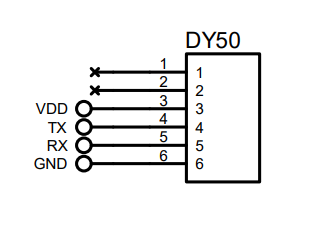
\includegraphics[width=0.3\textwidth]{figuras/eletronica/esquematicos/esq_conex_biometria.png}\label{fig:biometria_esq}}
        \caption{Sensor Biometria DY50}\label{fig:sensor_biometria}
    \end{figure}
    
    % \item Sensor de Leitura RFID
    \subparagraph*{$\bullet$ Sensor de Leitura RFID} \hfill
    
    O sensor de identificação por radiofrequência (RFID) utiliza um sistema de energização sem fio de etiquetas RFID para obtenção de dados armazenados nelas. Dessa forma, é utilizada uma antena que realiza a energização e captação desses dados numa frequência de 13,56 MHz, que posteriormente são decodificados e enviados por meio do protocolo I$^2$C para central de controle. 
    
    O uso do sensor RFID foi pensado para identificar os copos utilizados para armazenar as doses de medicamentos. Desse modo, sua identificação é necessária para determinar o copo que está recebendo a medicação. Para realizar a identificação e logística de distribuição de medicamentos para os pacientes, cada copo tem cores únicas para evitar ministração de doses medicamentosas para pacientes errados. 
    
    Com o posicionamento da etiqueta RFID na parte inferior do copo é possível ler sua identificação independentemente da face virada para o sensor. Uma vez que o sensor será posicionado entre as placas da esteira e o sensor poder identificar etiquetas RFID com uma distância determinada dependendo da antena utilizada. Como as placas da esteira utilizada são feitas de plástico, não ocorrerá problemas em relação a interferência na posição onde foi definido. 
    O modelo \textbf{PN532}, Fig. \ref{fig:sensor_RFID}, foi escolhido pela sua capacidade de distância de ativação das etiquetas chegar à 70 mm e sua antena pode ser modificada e direcionada para atender as necessidades de dimensionamento da máquina.
    
    A conexão do sensor de leitura RFID com a central de controle consiste em 4 pinos, esquemático na Fig. \ref{fig:sensor_RFID_esq}: VCC, GND, SDA e SCL, que são duas linhas de dados para comunicação I$^2$C. O componente, possui as seguintes especificações:
    
    \begin{itemize}
    \item[ ]
        \begin{itemize}
            \item Alimentação: 5 V;
            \item Interfaces: I$^2$C, SPI e \textit{High Speed UART} (HSU);
            \item Distância máxima de leitura/gravação: 70 mm;
            \item Preço: R\$ 33,99.
        \end{itemize}
    \end{itemize}
    
\begin{figure}[H]
    \centering
    \subfloat[][Sensor de leitura RFID PN532]{
    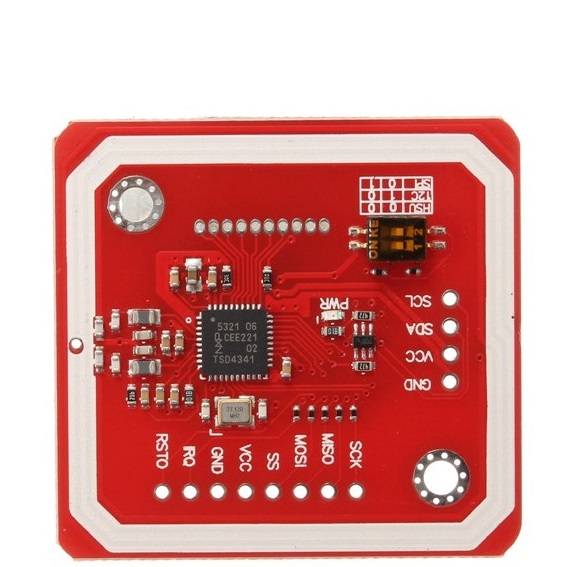
\includegraphics[width=0.25\textwidth]{figuras/eletronica/fotos_componentes/sensor_RFID.jpg}
    \label{fig:sensor_RFID}}
    \hspace{0.05\textwidth}
    \subfloat[][Conexões do módulo PN532]{
    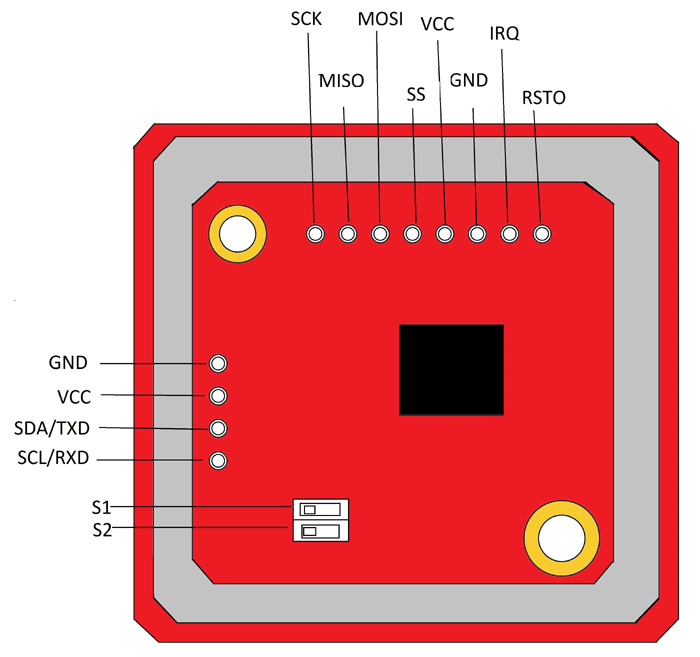
\includegraphics[width=0.25\textwidth]{figuras/eletronica/esquematicos/pinos_RFID.png}
    \label{fig:sensor_RFID_esq}}
    \caption{Módulo PN532}\label{fig:modulo_RFID}
\end{figure}
    
    O C.I. controlador RFID PN532 contempla um projeto de circuito com os componentes necessários para conectar uma antena, fornecido pelo fabricante. Este circuito RF consiste em 8 capacitores, 2 indutores, 2 resistores e a bobina de antena simétrica como mostrado na Fig. \ref{fig:antena_RFID}
    O filtro EMC reduz harmônicos de 13,56 MHz e executa uma impedância transformação. Em seguida, o circuito para casamento de impedâncias atua como um bloco de transformação de impedância. Por último, a própria bobina da antena gera o campo magnético, e assim recebe ou envia um sinal correspondente processado pelo PN532.
    
    \begin{figure}[H]
    \centering
    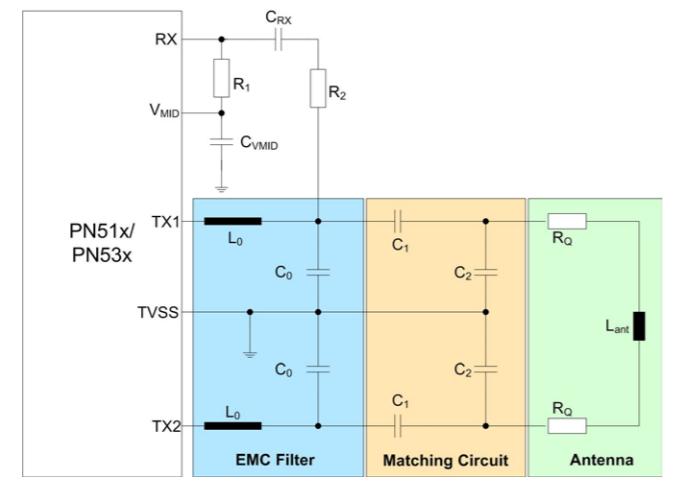
\includegraphics[scale=0.55]{figuras/eletronica/esquematicos/antena_RFID.png}
    \caption{Diagrama de blocos da parte RF}
    \label{fig:antena_RFID}
    \end{figure}

   Com base na escolha do módulo do sensor de leitura RFID com o PN532 integrado, nele existe uma antena seguindo o projeto do fabricante. Essa antena suporta a distância de até 70 mm para leitura e escrita em TAGs RFID compatíveis com a frequência de 13,56 MHz. Essa distância é suficiente para aplicação pois é superior a espessura do módulo da esteira utilizada, 19,9 mm indicada na Fig. \ref{fig:esteira} do apêndice \ref{cad_preliminar}.
   
   \subparagraph*{} $\bullet$ \textit{Tag} RFID \hfill
   
   Para escolha da \textit{tag} RFID, primeiro deve ser observado se ela é para o tipo de frequência do sensor RFID utilizado, neste caso 13,56 MHz. Em seguida, devemos ficar atentos para atender as dimensões e formato do copo utilizado. Pelas cotagens descritas na Fig. \ref{fig:copo} do apêndice \ref{cad_preliminar},  copo tem base com 55 mm de diâmetro e 1,5 mm de espessura. Por fim, é necessário ser compatível com uma distância mínima de 50 mm de leitura e escrita por variar dependendo do tamanho.
   
   Dessa forma foi escolhido a \textit{Tag} etiqueta RFID 13,56 MHz, representado na Fig. \ref{fig:etiqueta_rfid}. Ela tem diâmetro de 25 mm, menor que a base do copo, e suporta uma distância de comunicação de 50 mm, suficiente para aplicação.

    \begin{figure}[H]
        \centering
        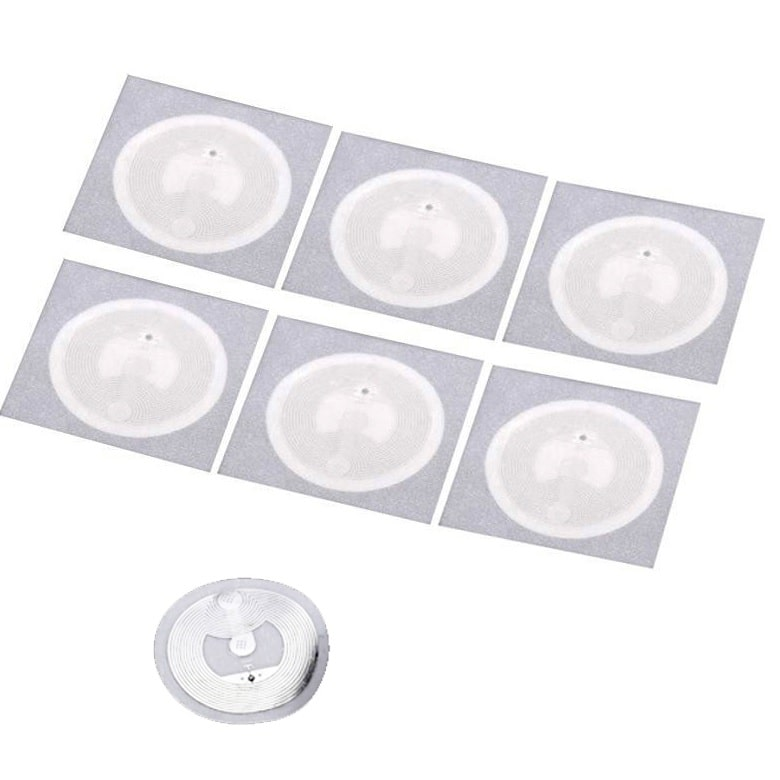
\includegraphics[width=0.3\textwidth]{figuras/eletronica/fotos_componentes/etiqueta_rfid.jpg}
        \caption{Tag etiqueta RFID 13,56 MHz}
        \label{fig:etiqueta_rfid}
     \end{figure}
%   Dessa forma, não será necessária a adição de uma outra antena para aumentar a distância de ativação das etiquetas, uma vez que, a antena embutida no módulo já contempla a distância necessária de 50mm para aplicação.
   
    % \item Câmera para Processamento de Imagens
    \subparagraph*{$\bullet$ Câmera para Processamento de Imagens} \hfill
    
    Atualmente câmeras estão presentes no dia-a-dia da população mundial, porém ainda mais presentes na automatização de processos industriais e verificação de qualidade por meio do processamento de imagens. Dessa forma, o uso de uma câmera foi escolhida para realizar a captação visual dos comprimidos. Posteriormente, a partir do  processamento dessas imagens, serão extraídas as características dos comprimidos, sendo possível identificar a quantidade e classificar o tipo de medicamento no copo de forma eficiente e confiável.
    
    A câmera escolhida foi a \textbf{OV5647}, Fig. \ref{fig:OV5647_pic}, por apresentar sensor com capacidade de gerar imagens de até 2592x1944 pixeis e preço acessível no Brasil. Ela utiliza o protocolo \textit{Camera Serial Interface} (CSI) para transmitir dados, sendo um padrão compatível para integração com a central de controle. Para realizar a conexão entre a câmera e a central de controle, especificamente o microprocessador utilizado, emprega-se um cabo \textit{flat} de 15 canais compatível com o soquete \textit{Zero Insertion Force} (ZIF) presente tanto no microprocessador como no módulo com a câmera OV5647, representação esquemática na Fig. \ref{fig:OV5647_esq}.
    
    \begin{figure}[H]
    \centering
    \subfloat[][Câmera OVN5647 com lente]{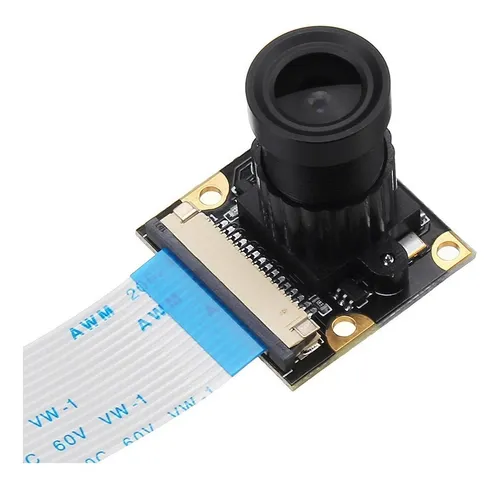
\includegraphics[width=0.25\textwidth]{figuras/eletronica/fotos_componentes/OV5647.png}\label{fig:OV5647_pic}}
    \hspace{0.1\textwidth}
    \subfloat[][Conexões CSI da Câmera OVN5647]{
    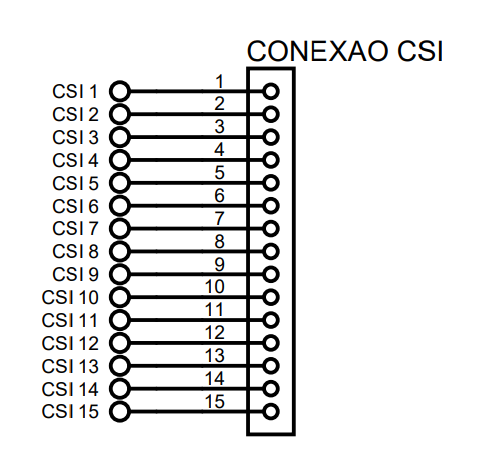
\includegraphics[width=0.25\textwidth]{figuras/eletronica/esquematicos/esq_conex_csi.png}\label{fig:OV5647_esq}}
    \caption{Câmera OV5647 - 5MP}\label{fig:camera_process}
    \end{figure}
    
    Para o processamento será aplicada uma técnica que consiste em detectar as bordas dos medicamentos. Com isso é criado máscaras binárias para cada comprimido identificado, isolando o comprimido e extraindo características do mesmo, como por exemplo, cor e formato.
    
    Após isso, será utilizado um classificador \textit{Support Vector Machine} (\textit{SVM}), treinado com uma biblioteca de imagens de comprimidos que tiveram as mesmas características extraídas. Sendo assim cruzados os dados dos comprimidos que eram previstos no copo com os dados do classificador \textit{SVM}, obtendo resultado positivo caso seja verificado que a dose está correta. 
    
    O classificador \textit{SVM} foi escolhido por ter solução determinística, não possuindo viés de treinamento e não demandando muitos recursos do sistema embarcado. 
% \end{itemize}

\section{Módulo de Acionamento de Atuadores}
     
    O Módulo de acionamento de atuadores tem a funcionalidade de controlar os atuadores contidos no dispositivo. Sendo assim, o módulo de acionamento de atuadores se trata de um sistema micro-controlado pela central de controle e são utilizados \textit{drivers} que controlam os atuadores do dispositivo. Estes seriam: motor DC, atuador, motores de passo, solenóides para os contêineres e as mini-travas elétricas solenóides em cada compartimento de acesso no sistema. 

% \begin{itemize}
%    \item Fechaduras
    % \item Drivers
    \subparagraph*{$\bullet$ \textit{Drivers}} \hfill
    
    Os \textit{drivers} dos atuadores são módulos projetados para prover a potência de atuação e a interação com o controle de forma simplificada. Eles convertem comandos por meio de portas lógicas em potência controlada para os atuadores. Dessa forma, tornam possível o controle automático de ações de movimento.
    
    \subparagraph*{} $\bullet$ \textbf{Motores de Passo}\label{sec:eletronica_drivers_passo}
    
    O \textit{driver} escolhido para os motores de passo é o módulo com C.I. \textbf{A4988} pois atende as características de carga para funcionamento do motor de passo escolhido, a partir da explicação na seção \ref{sec:energia_motor_passo} da solução energética. Além do mais, o \textit{driver} inclui a possibilidade de resolução do passo do motor em até 1/16 do considerado passo completo, assim o passo completo é o angulo mínimo, em graus, que o motor de passo realiza e é diferente para cada motor. No caso do motor escolhido, o passo completo segundo o fabricante é de 1,8$^\circ$. Por não ser uma aplicação que necessite de alta resolução para controle dos motores de passo, por apenas girar os fusos que rotacionam as engrenagens de um grupo de 5 contêineres até ser detectado a queda de um medicamento, a resolução de 1/16 do passo completo do motor é suficiente para controle.
    
    Para conexão entre a central de controle, especificamente o microcontrolador, e o \textit{driver} A4988 são utilizados 9 pinos:
    
    \begin{itemize}
        \item[ ]
        \begin{itemize}
            \item[ ]
            \begin{itemize}
                \item[$\bullet$] \textbf{VCC} e \textbf{GND} para alimentação da parte lógica.
                \item[$\bullet$] \textbf{MS1}, \textbf{MS2} e \textbf{MS3} são as portas lógicas que determinam a resolução do Passo: Passo Completo (estado lógico: ``000''); Meio Passo (estado lógico: ``100''); 1/4 Passo (estado lógico: ``010''); 1/8 Passo (estado lógico: ``001'');  1/16 Passo (estado lógico: ``111'').
                \item[$\bullet$] \textbf{\textit{ENABLE}} ativa (estado lógico: `1') ou desativa (estado lógico: `0') as saídas de tensão  e corrente para o motor de passo.
                \item[$\bullet$] \textbf{\textit{DIR}} Determina a direção de rotação do motor.
                \item[$\bullet$] \textbf{\textit{STEP}} Entrada de controle principal que cada transição de `0' para `1' realiza o movimento conforme a resolução determinada pelas portas MSx.
                \item[$\bullet$] \textbf{$\overline{\textbf{RESET}}$} quando vai para o estado lógico `0' ele reinicia o tradutor (bloco interno do C.I. que traduz as entradas de controle em tensões na saída para movimento do motor de passo) para um estado inicial pré-determinado e desativa todas as portas de saída para os motores. O \textit{driver} ignora todas as portas de entrada \textit{STEP} até ele voltar para o estado lógico `1' (desativado).
            \end{itemize}
        \end{itemize}
    \end{itemize}
    
    \newpage
    \subparagraph*{} $\bullet$ \textbf{Motor DC}
    
    O \textit{driver} escolhido para o motor DC é o \textbf{L298N}, seu controle é baseado na ponte H. Ele atende as especificações elétricas para alimentação do motor DC escolhido, explicado na seção \ref{energ:motor_dc} da solução energética. A estrutura de ponte H de eletrônica de potência permite a manipulação da tensão da fonte no motor por meio de chaveamento, dessa forma, é possível controlar a velocidade do motor. Para o chaveamento será utilizado o controle por modulação de pulso (\textit{PWM}), implementado na rotina do \textit{firmware} do microcontrolador. Essa tecnologia varia o tempo de permanência do sinal lógico em baixo e alto, isso acarreta uma resposta que simula uma variação de intensidade de tensão, porém variando apenas o tempo que o sinal está ligado.  
    
    Para conexão entre a central de controle, especificamente o microcontrolador, e a ponte H L298 são utilizados 3 pinos:
    
    \begin{itemize}
        \item[ ]
        \begin{itemize}
            \item[ ]
            \begin{itemize}
                \item[$\bullet$] \textbf{IN1} e \textbf{IN2} (Entrada 1 e Entrada 2) são as entradas de controle do motor na ponte H. São 4 possibilidades lógicas para esses pinos: ``00'' motor gira no sentido direto, ``01'' motor gira no sentido reverso, ``10'' freio do sentido direto e ``01'' freio do sentido reverso.
                \item[$\bullet$] \textbf{GND} para conectar as referências lógicas do microcontrolador e da ponte H.
            \end{itemize}
        \end{itemize}
    \end{itemize}
    
    
    \subparagraph*{ $\bullet$ \textbf{Solenoides e Atuador Linear}}
    
    O \textit{driver} escolhido para os solenoides e o atuador linear, foi o módulo com C.I. \textbf{IRF520N}, uma vez que, atende as características elétricas para funcionamento deles, explicado nas seções \ref{energ:solenoide} e \ref{energ:atuador_linear} da solução energética. E suas configurações possibilitam a utilização de sinais lógicos pelo microcontrolador para controle.
    
    Para conexão entre a central de controle, especificamente o microcontrolador, e o \textit{driver} IRF520N são utilizados 2 pinos:
    
        \begin{itemize}
        \item[ ]
        \begin{itemize}
            \item[ ]
            \begin{itemize}
                \item[$\bullet$] \textbf{SIGNAL} para o sinal lógico de controle por nível lógico.
                \item[$\bullet$] \textbf{GND} para referência da parte lógica.
            \end{itemize}
        \end{itemize}
    \end{itemize}
    
    % \item Isolamento
    % \subparagraph*{$\bullet$ Isolamento} \hfill
    
    % A natureza dos atuadores gera ruídos de tensão e corrente que devem ser tratados, uma vez que, caso esse ruído chegue ao sistema de controle existe a possibilidade de causar mal funcionamento das funções de todos os circuitos presentes. Portanto, deve-se isolar o sistema de atuadores do sistema de controle. Para isso são utilizados opto-acopladores, que isolam o sistema transferindo sinais por meio de \textit{LEDs} emissores e receptores.
    

\section{Central de Controle}

A central de controle é o sistema que irá realizar tanto a análise dos dados coletados no módulo de medição quanto o controle do sistema de atuadores do dispositivo. Bem como é por onde comandos são recebidos e enviados  no \textit{Backend} - nome que representa a parte da arquitetura de software que interage com a central de controle. 

O principal componente da central de controle é o computador de placa única. Adicionalmente  temos um meio para o usuário interagir com o sistema embarcado. Esta interação é feita pelo subsistema denominado módulo de visualização.

% \begin{itemize}
%     \item Microprocessadores
\subsection{Sistema Embarcado}\label{sec:sistema_embarcado}
    % \subparagraph*{$\bullet$ Microprocessadores}  \hfill
    \subparagraph*{$\bullet$ Computador de Placa Única}  \hfill
    
    A adoção de microprocessadores é bastante comum atualmente em implementações de sistemas embarcados nas mais diversas aplicações. Em especial temos diversos fabricantes que implementaram sistemas usando microprocessadores que tem suporte a um sistema operacional (SO) e inclua uma interface de entradas e saídas digitais com propósito geral, sendo denominadas como computadores de placa única (\textit{Single Board Computers} - SBCs). 
    
    % Alguns exemplos comuns no mercado são as placas \textit{Raspberry's Pi} desenvolvidas pela \textit{Raspberry Pi Foundation}, placas Tinker da ASUS, placas BeagleBoards da Texas Instruments e as placas NVIDIA Jetson da NVIDIA. 
    
    A utilização de uma \textit{SBC} é devido necessidade desse sistema desempenhar várias funções que necessitam do suporte de um computador com sistema operacional, realizando  operações para área eletrônica como: Processamento de imagens dos medicamentos; Interface gráfica do módulo de visualização; Captura de dados de múltiplos sensores; Controle dos atuadores.
    
    Também é necessário que o sistema utilizado tenha suporte a protocolos de comunicação I$^2$C, \textit{SPI}, \textit{UART} e \textit{CSI}, entre os módulos de medição e visualização e a central de controle. Principalmente, deve-se conter pinos GPIO para realizar a conexão física desses protocolos. Além do mais, é necessário que o sistema operacional escolhido tenha suporte as ferramentas e algoritmos de comunicação com as arquiteturas usadas na área de Software.
    
    Após uma análise de vários modelos comparando principalmente os componentes integrados como processador central (CPU), processador gráfico (GPU), tipo de memória RAM, quantidade de memória RAM, periféricos embarcados (tipo USB, módulo Wi/Fi, internet) e o preço relativo praticado em fornecedores no Brasil foi escolhido a \textbf{\textit{Raspberry Pi }4 B} com \textbf{4 GB DDR4}. 
    
    A \textit{Raspberry Pi} 4 tem suporte em \textit{hardware} para os protocolos de comunicação suportados para comunicação entre os componentes da central de controle e sensores específicos do módulo de medição. Ou seja, em seu GPIO existem conexão da comunicação I$^2$C, \textit{SPI}, \textit{UART}, sendo que para o protocolo \textit{CSI} é utilizado o soquete ZIF de 15 pinos na parte traseira da placa. 
    
    O armazenamento será suportado em hardware pela \textit{Raspberry Pi}, sendo empregado o cartão de memória chamado em inglês de \textit{Secure Digital Card} (SD Card). Para o tamanho do cartão de memória foi selecionado o de 32 Gb, já que não serão  armazenadas as imagens usadas no processamento de imagem e o banco de dados não armazena um grande volume de dados, apenas arquivos de Mbs e Kbs. Por fim, foi avaliado as especificações da velocidade de leitura e escrita do SD card em relação ao preço final. 
    
    Sendo assim, foi escolhido o SD Card \textbf{SanDisk Extreme} com \textbf{32 GBs} de armazenamento e especificação de leitura em até 100 MB/s e escrita de 90 MB/s. Além de atender os requisitos, essa escolha foi baseada em um comparativo de velocidade realizado pela impressa especializada aliada ao preço em fornecedores locais \cite{sdcard_benchmark}. 
    
    Para o sistema operacional foi escolhido o \textit{Ubuntu Server} 18.04.05 LTS por ser uma versão lançada em 2018 no mercado e seu ciclo de vida terminar em Abril de 2023. Assim, o ciclo de vida representa a data final em que a versão do sistema operacional para de receber suporte oficial da comunidade \textit{Ubuntu} para atualizações de segurança e novidades. Esses sistema operacional suporta todas as bibliotecas utilizadas para desenvolvimento da comunicação e controle dos subsistemas da eletrônica e da solução de software.
    
    % \item Microcontroladores
    \subparagraph*{$\bullet$ Microcontroladores} \hfill
    
    Os microcontroladores são utilizados nas mais diversas aplicações de controle e automação. Assim, os microcontroladores possuem os itens essenciais de processamento, aliados a periféricos abundantes para entradas e saídas de dados com um  baixo custo, possibilitam o desenvolvimento de sistemas robustos e escaláveis.
    
    % Melhor 
    Segundo John Morton \cite{morton2005pic}, para escolha do microcontrolador primeiro deve ser realizado um rascunho do projeto, observando o que será feito e o que o microcontrolador deve fazer. O próximo passo deve ser realizado um diagrama do circuito ou representação similar, vendo em particular todas as entradas e saídas necessárias para conectar com o microcontrolador atendem aos requisitos do projeto, sendo um dos principais fatores de escolha devido a limitação de porta que cada microcontrolador possui. Como, por exemplo, PIC16F54 tem até 12 pinos entrada/saída (em inglês \textit{input/output} - I/O) e a PIC16F57 até 20.
    
    Dado a metologia de escolha, temos que em nosso projeto os microcontroladores serão utilizados para direcionar dados do módulo de medição para o sistema microprocessado e o mesmo enviar dados de controle para o módulo de acionamento de atuadores. Para direcionamento desses dados entre os microcontroladores e o sistema microprocessado escolhido (\textit{Raspberry Pi} 4) foi determinado o uso do protocolo I$^2$C, sendo assim um requisito para escolha do microcontrolador.
    
    Para determinação da quantidade de pinos primeiro devemos listar a quantidade de cada componente conectado aos microcontroladores e os pinos necessários para cada unidade, excluindo pinos de alimentação como +5 V e GND e observando se os pinos utilizados atendem a como o dado vem do sensor, ou seja, se é digital ou é necessário o uso de uma porta com conversão analógico-digital. Na Tab. \ref{tab:pinos_microcontrolador} está a compilação da quantidade total de pinos necessários.
    
    \begin{table}[H]
    \centering
    \caption{Levantamento da quantidade de pinos}
    \label{tab:pinos_microcontrolador}
    \begin{adjustbox}{max width = \textwidth}
        \begin{tabular}{|L{5cm}|C{2cm}|C{2cm}|C{2cm}|C{2cm}|C{2cm}|}
            \hline
            \rowcolor[HTML]{A8DADC}
            \textbf{Componente} & \textbf{Quantidade} & \textbf{Pinos (unid.)} &  \textbf{Tipo} & \textbf{Pinos (Total)}  \\ \hline
            % Sensor de Temperatura e Umidade & 1	 & 3,3 & 0,0005 & 0,0015
            % \\ \hline
           %   Sensor Fotoelétrico Emissor & 30	 & 3,3 & 0,1 & 9,9
         %   \\ \hline
              Sensor de Barreira & 30 & 1  & I/O & 30
             \\ \hline
             Chave Micro \textit{Switch} & 33 & 1 & I/O & 33
            \\ \hline
             Teclado & 1 & 1 & Analógico & 1
            \\ \hline
            %  Cls Mux/Demux & 12 & 5 & 0,000001 & 
            % \\ \hline
               \textit{Driver} A4988 & 5 & 7 & I/O & 35
             \\ \hline
               \textit{Driver} IRF520N & 33 & 1 & I/O & 33
             \\ \hline
               \textit{Driver} Ponte H L298 & 1 & 2 & I/O & 2
             \\ \hline
             \rowcolor[HTML]{F1FAEE}
             \multicolumn{4}{|l|}{\cellcolor[HTML]{F1FAEE}Total} & 133 \\
             \hline
        \end{tabular}
    \end{adjustbox}
\end{table}
    \subparagraph*{Nota:} Está sendo levado em consideração que o visor LCD, o sensor de biometria DY50, o sensor RFID PN532, o sensor de temperatura e umidade HTU21D e a câmera não se conectam aos microcontroladores.
    
    %alterar
    Analisando a Tab. \ref{tab:pinos_microcontrolador} pode-se concluir que os componentes com maior quantidade são os sensores de barreira (30 un.), as chaves (33 un.) e os \textit{drivers} IRF520N(33 un.), totalizando 95 componentes. Como o controle foi desenvolvido para que a medição ou controle para os componentes de mesmo tipo não seja paralela é possível simplificar como eles são conectados a central de controle, descrição do controle se encontra na seção \ref{sec:rede_petri}. Desse modo, pode-se utilizar multiplexadores e demultiplexadores (MUX/DEMUX) para diminuir a quantidade de portas de I/O conectadas de sensores de barreira, chaves e \textit{drivers} IRF520N com o microcontrolador. Sendo assim foi escolhido MUX/DEMUX 8x1, especificamente pelo uso do CI CD4051. 
    
    O CD4051 é um C.I. de multiplexação ou demultiplexação com 13 pinos: 
    
    \begin{itemize}
        \item 8 pinos de entradas/saídas;
        \item 1 pino de saída/entrada;
        \item 3 pinos para chaveamento de qual dos oito canais são as saídas;
        \item 1 pino \textit{ENABLE} que desliga o funcionamento do C.I.
    \end{itemize}
    
    Levando em consideração os 13 pinos de um MUX/DEMUX foi calculado a razão de redução de pinos. Para isso é levado em consideração que, para o mesmo tipo de componente, é utilizado a quantidade mais próxima de MUX/DEMUX a quantidade total do componente sem deixar sobrar portas entrada ou saída no MUX/DEMUX. Em seguida, foi considerado que os 3 pinos de chaveamento são conectados aos mesmos 3 pinos no microcontrolador, independente da quantidade utilizada de C.I.s. E os pinos de saída/entrada do MUX/DEMUX e \textit{ENABLE} tem conexão individual no multiplexador. Por fim calculamos a razão de redução pela Eq. \ref{eq:reducao_pins}.
    
    \begin{equation}\label{eq:reducao_pins}
        \text{Razão de Redução de Pinos (RRP)} = \frac{\text{Quantidade final}}{\text{Quantidade Inicial}}
    \end{equation}
    
    Onde Quantidade final é o total de pinos conectados ao microcontrolador após o uso dos MUX/DEMUX 8x1 e a Quantidade inicial é o total de pinos conectados determinado na Tab. \ref{tab:pinos_microcontrolador}. Seguindo a metodologia descrita e aplicando a Eq. \ref{eq:reducao_pins} para os 3 componentes com maior quantidade obtemos:
    
    \begin{itemize}
        \item \textbf{Sensores de Barreira:} 30 unidades sendo 24 conectadas a 3 multiplexadores (necessário $3 + 3\cdot2 = 9$ pinos) e 6 diretamente no microcontrolador. 
        
        $RRP = \frac{(9 + 6)}{30} = 0.5$
        
        \item \textbf{Chaves tipo Micro \textit{Switch}:} 33 unidades sendo 32 conectadas a 4 multiplexadores (necessário $3 + 4\cdot2 = 11$ pinos) e 1 diretamente no microcontrolador. 
        
        $RRP = \frac{(11 + 1)}{33} = 0.36$
        
        \item \textbf{\textit{Driver} IRF520N:} 33 unidades sendo 32 conectadas a 4 multiplexadores (necessário $3 + 4\cdot2 = 11$ pinos) e 1 diretamente no microcontrolador. 
        
        $RRP = \frac{(11 + 1)}{33} = 0.36$
        
    \end{itemize}
    
    Recalculando o total de pinos necessários nos microcontroladores ocorreu uma redução de 96 para 39 para os 3 componentes de maior quantidade (sensores de barreira, chaves e \textit{driver} IRF520N). 
    
    Analisando o \textit{driver} A4988, usado para os motores de passo, é necessário um total de 35 pinos. Com a funcionalidade de cada conexão explicada na seção \ref{sec:eletronica_drivers_passo}, pode-se simplificar sua conexão aos microcontroladores pois apenas um vai funcionar por vez e todos realizam o mesmo tipo de movimento. Assim, dos 7 pinos utilizados para cada \textit{driver} A4988, 6 podem estar conectados na mesma porta lógica do microcontrolador para os 5 utilizados. Onde a porta de \textit{ENABLE} de cada \textit{driver} tem conexão individual com o microcontrolador. Ou seja, para os 5 utilizados para controle dos motores de passo são necessários 6 pinos (portas comuns entre os \textit{drivers}) e 5 pinos \textit{ENABLE} para cada um. Proporcionando a diminuição do total de 35 para 11 pinos necessários para os \textit{drivers} A4988.
    
    Com todas as simplificações de conexão aos microcontroladores descritas a quantidade total de pinos necessária diminuiu de 133, conforme Tab. \ref{tab:pinos_microcontrolador}, para 53 ($39 + 11 + 1 + 2 = 53$).
    
    Para evitar qualquer ruído inerente dos atuadores serão usados microcontroladores exclusivos tanto para o módulo de acionamento dos atuadores quanto para o módulo de medição. Desse modo, é garantida uma integridade dos valores medidos dos sensores no módulo de medição.
    
    Sendo assim, realiza-se a separação dos pinos por tipo de sistema em que está conectado (módulo de medição ou módulo de acionamento de atuadores). Os componentes com maior quantidade (sensores barreira, chaves e \textit{driver} IRF520N), os pinos de conexão são adicionados para o protocolo de comunicação I$^2$C (2 pinos - SDA e SCL) é necessário 4 microcontroladores com pelo menos 15 pinos. Onde um deles precisa ter uma entrada com conversor A/D para a conexão analógica do teclado. 
    
    Com a funcionalidade do microcontrolador determinada, a quantidade e os tipo de pinos necessários e a quantidade de microcontroladores foi decidido usar os da família PIC, fabricados pela \textit{Microchip Technology}. Sua arquitetura foi escolhida por ser compatível com bibliotecas de leitura, comunicação e controle dos \textit{drivers} dos atuadores. Também existe a disponibilidade em fornecedores locais de uma variedade de C.I.s de microcontroladores com diferentes quantidade de pinos I/O, conversão A/D de várias resolução e comunicação I$^2$. Sendo  possível a criação de circuitos customizados para aplicação sem a necessidade utilização de placas de desenvolvimento de microcontroladores, como Arduino UNO ou MSP430. Sendo assim, o microcontrolador escolhido foi o \textbf{PIC16F677} por conter 17 pinos I/O, onde 2 podem ser configurados para comunicação I$^2$C, 12 podem ser configurados como conversor A/D de 10 bits e pode ser alimentado com uma tensão de 5 V, compatível com as duas possibilidades disponíveis pela solução energética.

% \item Módulo de Visualização
    % \subparagraph*{$\bullet$ Módulo de Visualização} \hfill

\subsection{Módulo de Visualização}
    
    O módulo de visualização é o subsistema onde o usuário poderá visualizar algumas informações úteis de funcionamento e gestão do dispositivo e interagir com essa interface usando as teclas de interação. Nele estão contidos um visor e um teclado para interface com o usuário.
    
    No apêndice \ref{app_telas_display} consta o \textit{mockup} desenvolvido para as telas presentes na interface.
 
    % \begin{itemize}
    %     \item Visor 
        \subparagraph*{}$\bullet$ \textbf{Visor} \hfill
        
        Existem diversas tecnologias de visor disponíveis no mercado que podem ser utilizadas no projeto. Para delimitação do visor foi levado em consideração compatibilidade do protocolo de comunicação com sistema microprocessado escolhido, tamanho da visor, tecnologia de visor para visualização nas cores RGB e preço relativo. Sendo assim foi escolhido o visor tipo LCD TFT de 3,2'' com as seguintes características:
        
        \vspace{-0.2cm}
        \begin{itemize}
            \item[ ] 
            \begin{itemize}
            \item \textbf{Visor:} Tipo LCD TFT 3,2'' 
            \item \textbf{Controlador:} ILI9341
            \item \textbf{Resolução:} 240x320 pixeis;
            \item \textbf{Dimensões do visor:} 48,60 x 64,80 mm
            \item \textbf{Interface:} SPI
            \end{itemize}
        \end{itemize}
        
        % \vspace{-0.2cm}
        
        \begin{figure}[H]
        \centering
        \subfloat[][Visor tipo LCD TFT]{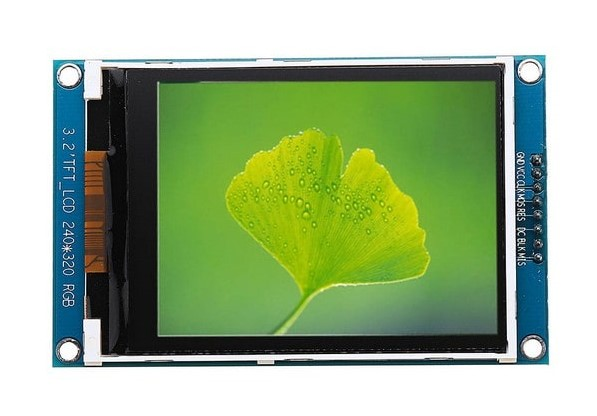
\includegraphics[width=0.4\textwidth]{figuras/eletronica/fotos_componentes/Display-LCD-TFT-3.2-240x320-6.jpg}\label{fig:LCD_pic}}
        \hspace{0.1\textwidth}
        \subfloat[][Conexões do visor LCD - Protocolo SPI]{
        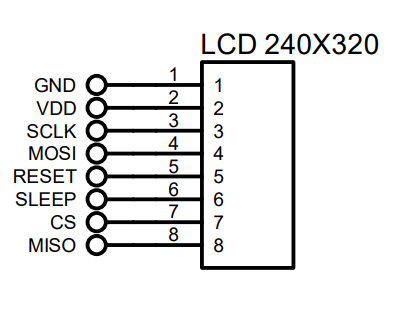
\includegraphics[width=0.365\textwidth]{figuras/eletronica/esquematicos/esq_lcd_320.png}\label{fig:LCD_esq}}
        \caption{Visor tipo LCD TFT 240x320}
        \label{fig:display_lcd}
        \end{figure}
        
        % \item Teclado
        \subparagraph*{$\bullet$ \textbf{Teclado}} \hfill
        
        A utilização de uma matriz de botões é necessária para o usuário do dispositivo poder interagir com os menus de opções disponíveis no visor de visualização. Neste caso foi preferível o uso de botões, uma vez que todos os cadastros de medicação, paciente, enfermeiro serão realizados pelo aplicativo e a interação no dispositivo é limitada a funções básicas como configurações internas do dispositivo e quando há falta de internet. 
        
        
        Sendo assim será usado uma configuração de arquitetura chamada de matriz de botões, especificamente uma solução comercial \textit{AdKeypad} com 5 botões como na Fig. \ref{fig:keypad_ft}.
        
        \begin{figure}[H]
          \centering
          \begin{minipage}[b]{0.3\textwidth}
            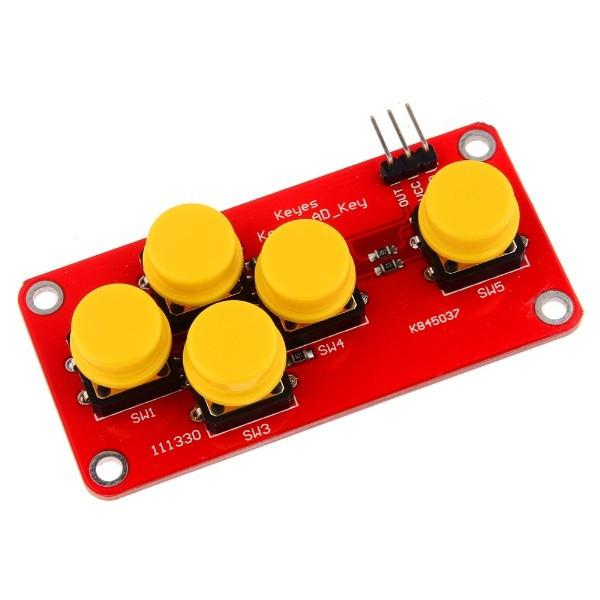
\includegraphics[width=\textwidth]{figuras/eletronica/fotos_componentes/adkeypad.jpg}
            \caption{\textit{AdKeypad} com 5 botões}
            \label{fig:keypad_ft}
          \end{minipage}
          \hspace{2cm}
          \begin{minipage}[b]{0.295\textwidth}
            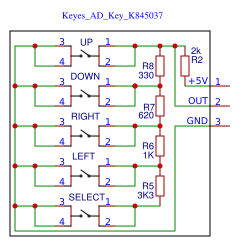
\includegraphics[width=\textwidth]{figuras/eletronica/esquematicos/adkeypad_schematic.png}
            \caption{Esquemático \textit{AdKeypad}}
            \label{fig:keypad_esq}
          \end{minipage}
        \end{figure}
        
        Analisando o circuito esquematizado na Fig. \ref{fig:keypad_esq} pode-se calcular a saída de tensão do circuito dependendo do tipo de tecla que é clicada. O circuito se comporta como vários divisores de tensão, onde a resistência varia dependendo da tecla que é clicada. Assim obtemos a Eq. \ref{eq:teclado}, que representa o cálculo da tensão $V_{out}$ seguindo as entradas e saídas da Fig. \ref{fig:keypad_esq}.
        
        \begin{equation}\label{eq:teclado}
            V_{out} = \frac{R_{EQ}}{R_2 + R_{EQ}} \cdot V_{in} \quad [\text{V}]
        \end{equation}
        
        Onde $V_{in}$ é a tensão de alimentação (5 V), $R_2$ é o resistor de 2 k$\Omega$ e $R_{EQ}$ é a soma dos resistores $R_8$, $R_7$, $R_6$ e $R5$ dependendo da tecla que está sendo clicada. Sendo assim temos o resultado de $V_{out}$ na Tab. \ref{tab:teclado}.
        
        \begin{table}[H]
        \centering
        \caption{Resultado para tensão $V_{out}$}
        \label{tab:teclado}
        \begin{adjustbox}{max width = \textwidth}
            % \begin{tabular}{|L{5cm}|C{2cm}|C{2cm}|C{2cm}|C{2cm}|C{2cm}|}
            \begin{tabular}{|l|c|c|c|}
                \hline
                \rowcolor[HTML]{A8DADC}
                \textbf{Tecla} & $R_2$ [k$\Omega$] & $R_{EQ}$ [$\Omega$] & $V_{out}$ [V] \\ \hline
                \textit{CIMA} & 2 & x & 0 \\ \hline
                \textit{BAIXO} & 2 & 330  & 0,708 \\ \hline
                \textit{DIREITA} & 2 & 950 & 1,610 \\ \hline
                \textit{ESQUERDA} & 2 & 1950 & 2,468 \\ \hline
                \textit{SELECIONA} & 2 & 5250 & 3,621 \\ \hline
                % Sensor de Temperatura e Umidade & 1	 & 3,3 & 0,0005 & 0,0015
            \end{tabular}
        \end{adjustbox}
        \end{table}
            
        Sua comunicação com microcontrolador é do tipo analógica, fazendo com o que o microcontrolador necessite de uma entrada com conversor analógico digital para que seja realizada a leitura dos dados provenientes do teclado. Conforme o esquemático, na Fig. \ref{fig:keypad_esq}, pode-se observar que existe apenas um pino de dados (2) para esse teclado. A central de controle irá interpretar qual botão foi pressionado a partir do sinal digital resultante da conversão analógica digital da tensão de saída, determinada na Tab. \ref{tab:teclado}, no pino de dados (2). 
        
        % Ver se mantem ou nao
        % Essa conversão é realizada em um microcontrolador, na qual o pino (2) de dados será conectado a uns dos pinos A/D de um dos microcontroladores que são usados no módulo de medição.
        
        %% Mais escrita 
        
        % Escrever sobre conversor analógico digital, escrevendo os resultados conforme esquematico do microcontrolador e calculando o erro (se necessário)
        
        %metodologia de erros nos sensores tanto analógico quanto no conversor a/d do microcontrolador - quantificação de erro bibliotecas de correção de erro de software
        
    % \end{itemize}

% \end{itemize}
\section{Protocolos de comunicação}
\subsection{Protocolos internos}

Os protocolos internos são aqueles utilizados para comunicação entre os subsistemas e componentes da solução eletrônica.

\begin{itemize}
    \item I$^2$C
    
    O protocolo I$^2$C descreve o funcionamento de um barramento serial que opera com dois fios, o SCL que é responsável por levar o \textit{clock} do dispositivo mestre para os dispositivos escravos e o SDA para a transferência de dados. Assim, para iniciar uma comunicação com escravos, o mestre coloca o valor lógico da linha SDA em baixo e logo em seguida é enviado o endereço do escravo que será utilizado. 
    
    Se o dispositivo escravo existir naquele endereço, um sinal de nível baixo é enviado pelo canal SCL após o oitavo pulso de \textit{clock}. Após isso, o mestre lê ou escreve nos registradores selecionados do escravo. Ou seja, é uma comunicação bidirecional. 
    
    Na aplicação proposta este protocolo é usado para comunicação do dispositivo mestre, sistema microprocessado (\textit{Raspberry Pi} 4), com dispositivos escravos. Os escravos são os quatro microcontroladores PIC16F677, o sensor de temperatura/umidade e o sensor RFID.
    
    \begin{figure}[H]
    \centering
    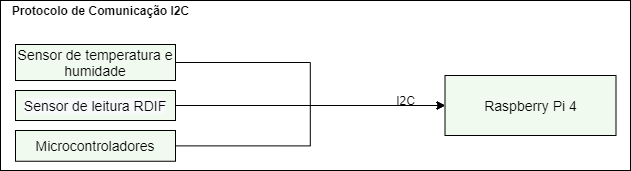
\includegraphics[width=0.7\textwidth]{figuras/eletronica/fluxogramas/comunicacao_i2c.png}
    \caption{Comunicação I$^2$C}
    \label{fig:PC_i2c}
\end{figure}
    
    \item SPI
    
    O protocolo SPI possui três fios fixos e um adicional para cada escravo no sistema. Sua comunicação é unidirecional em cada fio de comunicação, sendo o MOSI (\textit{Master Output Slave Input}) partindo do mestre para o escravo, o MISO (\textit{Master Input Slave Output}) partindo do escravo para o mestre, e o SCLK que é o \textit{clock} serial do mestre. Para controlar qual escravo está sendo usado, é empregado o pino de seleção de escravo SS, que precisa de um nível baixo para operar. Por mais que este protocolo precise de mais canais para seu funcionamento, as velocidades alcançadas  superam as do I$^2$C pois a deformação do sinal é menor pelo uso de transistores definindo o estado do pino (Push-Pull) ao invés de dreno aberto (Pull-Up).
    
    O protocolo SPI é utilizado para comunicar o dispositivo mestre, sistema microprocessado, com o visor LCD TFT 240x320. Devido a ser o protocolo compatível com o controlador do visor escolhido.
    
\begin{figure}[H]
    \centering
    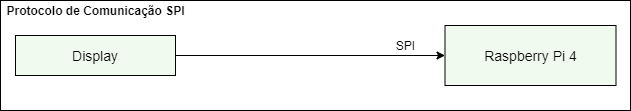
\includegraphics[width=0.7\textwidth]{figuras/eletronica/fluxogramas/comunicacao_spi.png}
    \caption{Comunicação SPI}
    \label{fig:PC_SPI}
\end{figure}

    \item UART
    
    O protocolo UART utiliza dois canais de comunicação, o RX para receber os dados e o TX para enviar. Esse protocolo trabalha de forma assíncrona, necessitando de que o transmissor e o receptor estejam numa mesma taxa de transmissão (em inglês \textit{baudrate}).
    
    As conexões são feitas invertendo-se os canais em dois dispositivos distintos, ou seja, o canal TX é conectado no RX e vice-versa. Para iniciar uma transmissão é enviado um bit de início, seguido de cinco a nove bits de informação, um bit de paridade e um a dois bits de finalização de transmissão.
    
    Este protocolo é usado para comunicar o dispositivo mestre, o sistema microprocessado, com o sensor de biometria DY50.
    
\begin{figure}[H]
    \centering
    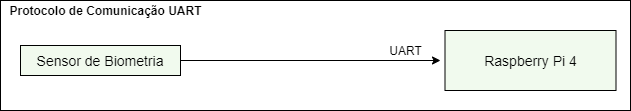
\includegraphics[width=0.7\textwidth]{figuras/eletronica/fluxogramas/comunicacao_uart.png}
    \caption{Comunicação UART}
    \label{fig:PC_UART}
\end{figure}
    
    \item CSI
    
    O protocolo CSI (\textit{Camera Serial Interface}) é caracterizado por uma fusão entre os protocolos I$^2$C e SPI. Ele utiliza duas interfaces, a primeira com os canais SCL e SDA para controle da câmera e a segunda com um canal de transmissão unidirecional da câmera para o processador e um canal de \textit{clock} da câmera para o processador.
    
    Este protocolo é o utilizado para comunicação entre a \textit{Raspberry Pi} 4 e o módulo com câmera OV5647.
    
\begin{figure}[H]
    \centering
    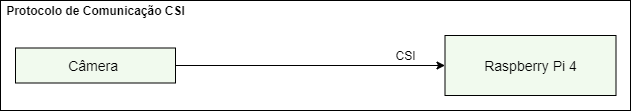
\includegraphics[width=0.7\textwidth]{figuras/eletronica/fluxogramas/comunicacao_csi.png}
    \caption{Comunicação CSI}
    \label{fig:PC_CSI}
\end{figure}
    
\end{itemize}
\subsection{Protocolos externos}

Os protocolos externos são aqueles utilizados para comunicação entre os sistemas de controle e alimentação do dispositivo com o \textit{back-end} da solução de software, esse é melhor detalhado \ref{sec:software_backend}.

\begin{itemize}
    \item HTTP
    
    O protocolo HTTP será utilizado para requisições de dados do sistema embarcado para o \textit{back-end}. As informações requisitadas serão relacionadas a dados de funcionamento do sistema, como horários de medicação e dados de posicionamento dos medicamentos no sistema. Logo, será uma comunicação unidirecional feita do sistema embarcado para o \textit{back-end}.
    
    \item MQTT
    
    O protocolo MQTT será utilizado para comandos e confirmações, dessa forma é possível realizar requisições do \textit{back-end} para ações na máquina, como cadastro de enfermeiros ou reposição de remédios. Portanto existem  tópicos dedicados a enviar confirmações de que as ações requisitadas foram realizadas e atualizações de dados da máquina para o \textit{back-end}.
    
    
\end{itemize}

\section{Diagramas Esquemáticos da Conexão dos Sistemas}\label{sec:esq_conec_sistemas}

Os diagramas esquemáticos das conexões entre os componentes dos sistemas da solução eletrônica se encontram detalhados nos Esquemáticos Eletrônicos no apêndice \ref{esquematicos_eletronica}.

\section{Arquitetura de Eletrônica}\label{sec:arq_eletronica}

No diagrama lógico da arquitetura geral da eletrônica na Fig. \ref{fig:fluxograma_eletronica} tem-se a interação dos módulos de medição com a central de controle e a interação do módulo de acionamento dos atuadores com a central de controle. Essa comunicação interna do dispositivo está explicada e esquematizada no apêndice \ref{esquematicos_eletronica}. Além do mais, nesse fluxograma é apresentada a alimentação necessária para cada componente.


\begin{figure}[H]
    \centering
    % \begin{adjustbox}{max width = \textwidth}
    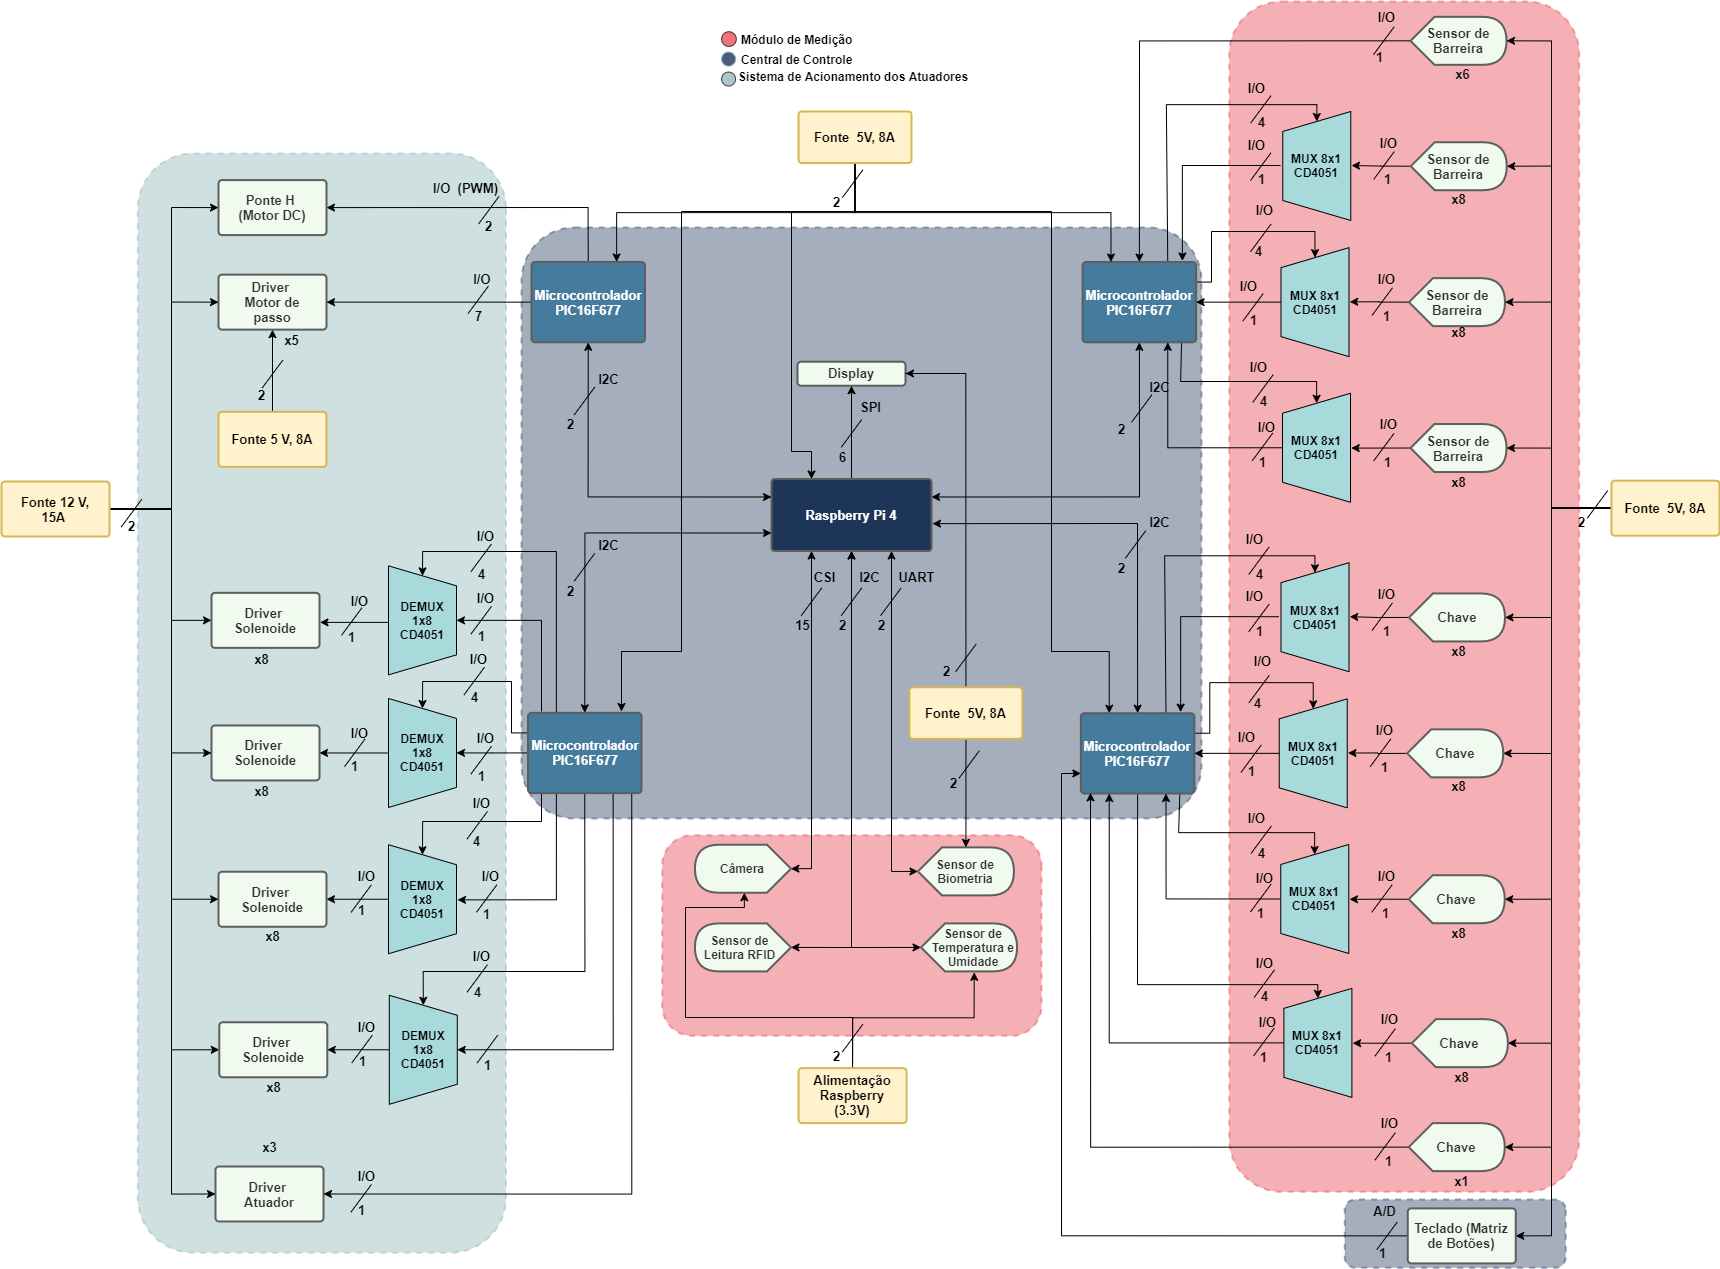
\includegraphics[width=1.1\textwidth]{figuras/eletronica/fluxogramas/fluxograma_eletronica.png}
    \caption{Diagrama Lógico Eletrônico}
    \label{fig:fluxograma_eletronica}
    % \end{adjustbox}
\end{figure}



\section{Rede de Petri}\label{sec:rede_petri}

A Rede de Petri é uma técnica de modelagem, a qual permite a representação de sistemas com embasamento matemático, e assim relaciona causa e efeito entre os eventos e as condições. Os elementos básicos que formam a topologia da redes de Petri são:
\begin{itemize}
    \item \textbf{Estados:} são usados para modelar os componentes passivos dos sistemas, correspondendo às variáveis de estado, no diagrama são representadas por círculos.
    \item \textbf{Ações:} são usadas para modelar os componentes ativos dos sistemas, são 
    os eventos de transição de um estado para outro, no diagrama são representadas por retângulos.
    \item \textbf{Fluxo:} através das ações do sistema é especificado como é a transformação de um estado para outro, no diagrama são representados por setas.
\end{itemize}

A partir do fluxograma de operação do sistema mecânico na Fig. \ref{fig:FEst}, representado na solução de estrutura na seção \ref{sec:dinamica_operacao}, elabora-se a Rede de Petri para representar e modelar o controle do dispositivo. 

Antes de iniciar o processo de controle os medicamentos são retirados das embalagens e são posicionados nos contêineres. Além do mais, os copos esterilizados também são dispostos no local de armazenamento dentro do dispositivo. A partir da Rede de Petri, na Fig. \ref{fig:rede_petri},  percebe-se que ocorrem dois processos em paralelo a separação do medicamento e o posicionamento do copo na esteira. 

O primeiro processo tem início com o medicamento sólido no contêiner, no qual cai na comporta com a ativação do \textit{driver} do motor de passo. O medicamento é detectado pelo sensor fotoelétrico de barreira e, em seguida, deve-se desativar o drive do motor de passo quando ocorrer a detecção para que não caia mais de um medicamento na comporta. Posteriormente, o solenoide é ativado para abrir a comporta. Quando a comporta é aberta o medicamento se desloca pelo canal de distribuição e, consequentemente, o solenoide é desativado. Em seguida, logo no final do funil do canal de distribuição, existe um sensor fotoelétrico de barreira para detectar a passagem do medicamento. Entretanto, quando o medicamento não é detectado pelo sensor, tem-se um aviso no visor do dispositivo que o medicamento está preso no dispositivo.

Enquanto isso, o outro processo em paralelo tem início com o copo no local de armazenamento. Sendo assim, no final do reservatório de copos está posicionado um sensor de barreira para verificar e detectar a passagem do copo. Logo, quando o copo é detectado deve-se ativar o \textit{driver} do atuador. Em seguida, quando o atuador é ativado, o copo é empurrado para a esteira e o \textit{driver} do atuador é desativado. Quando o copo está na esteira, é realizada a leitura da etiqueta RFID e os medicamentos são dispostos no copo a partir do posicionamento do copo abaixo do funil. Dessa forma, em uma dose medicamentosa que envolva mais de um comprimido o copo fica esperando até atingir o final do processo de separação dos medicamentos.

Posteriormente, quando ocorre a queda de todos os medicamentos da dose individual do paciente, o \textit{driver} da esteira é ativado e ela rotaciona para o sentido horário. Sendo assim, quando o copo com os medicamentos é detectado por outro sensor fotoelétrico de barreira, o qual é posicionado logo abaixo da câmera, o \textit{driver} da esteira é desativado e a esteira para, com a finalidade de realizar o captura das imagens para o processamento de imagem. 

Quando o processamento de imagens da dose individual conclui que existem erros de quantidade ou seleção, a esteira é ativada com o movimento anti-horário até chegar em outro sensor de barreira. Esse sensor detecta que o copo com medicamento caiu no compartimento de doses medicamentosas erradas. Caso contrário, quando a quantidade e a seleção de medicamentos estão corretas, a esteira é ativada com o movimento horário até chegar sensor de barreira que detecta que o copo está na zona de entrega e que o medicamento foi retirado do dispositivo. 

Portanto, quando existe um horário que mais de um paciente necessita da administração da medicação, a dose de medicamentos individuais é realizada sequencialmente para cada paciente. Quando é detectado que o copo está na zona de entrega o dispositivo retorna para a posição inicial para a nova sequência de dose individual.

No processo de reabastecimento, em que é necessário abrir a comporta superior para adição de medicamentos e retirar os contêineres para limpeza, utiliza-se uma chave. Com ela é possível detectar se a porta está fechada e se os contêineres estão corretamente encaixados. Caso contrário, deve-se enviar um aviso no visor para que o enfermeiro possa corrigir essas anomalias. 

\begin{figure}[H]
    \centering
    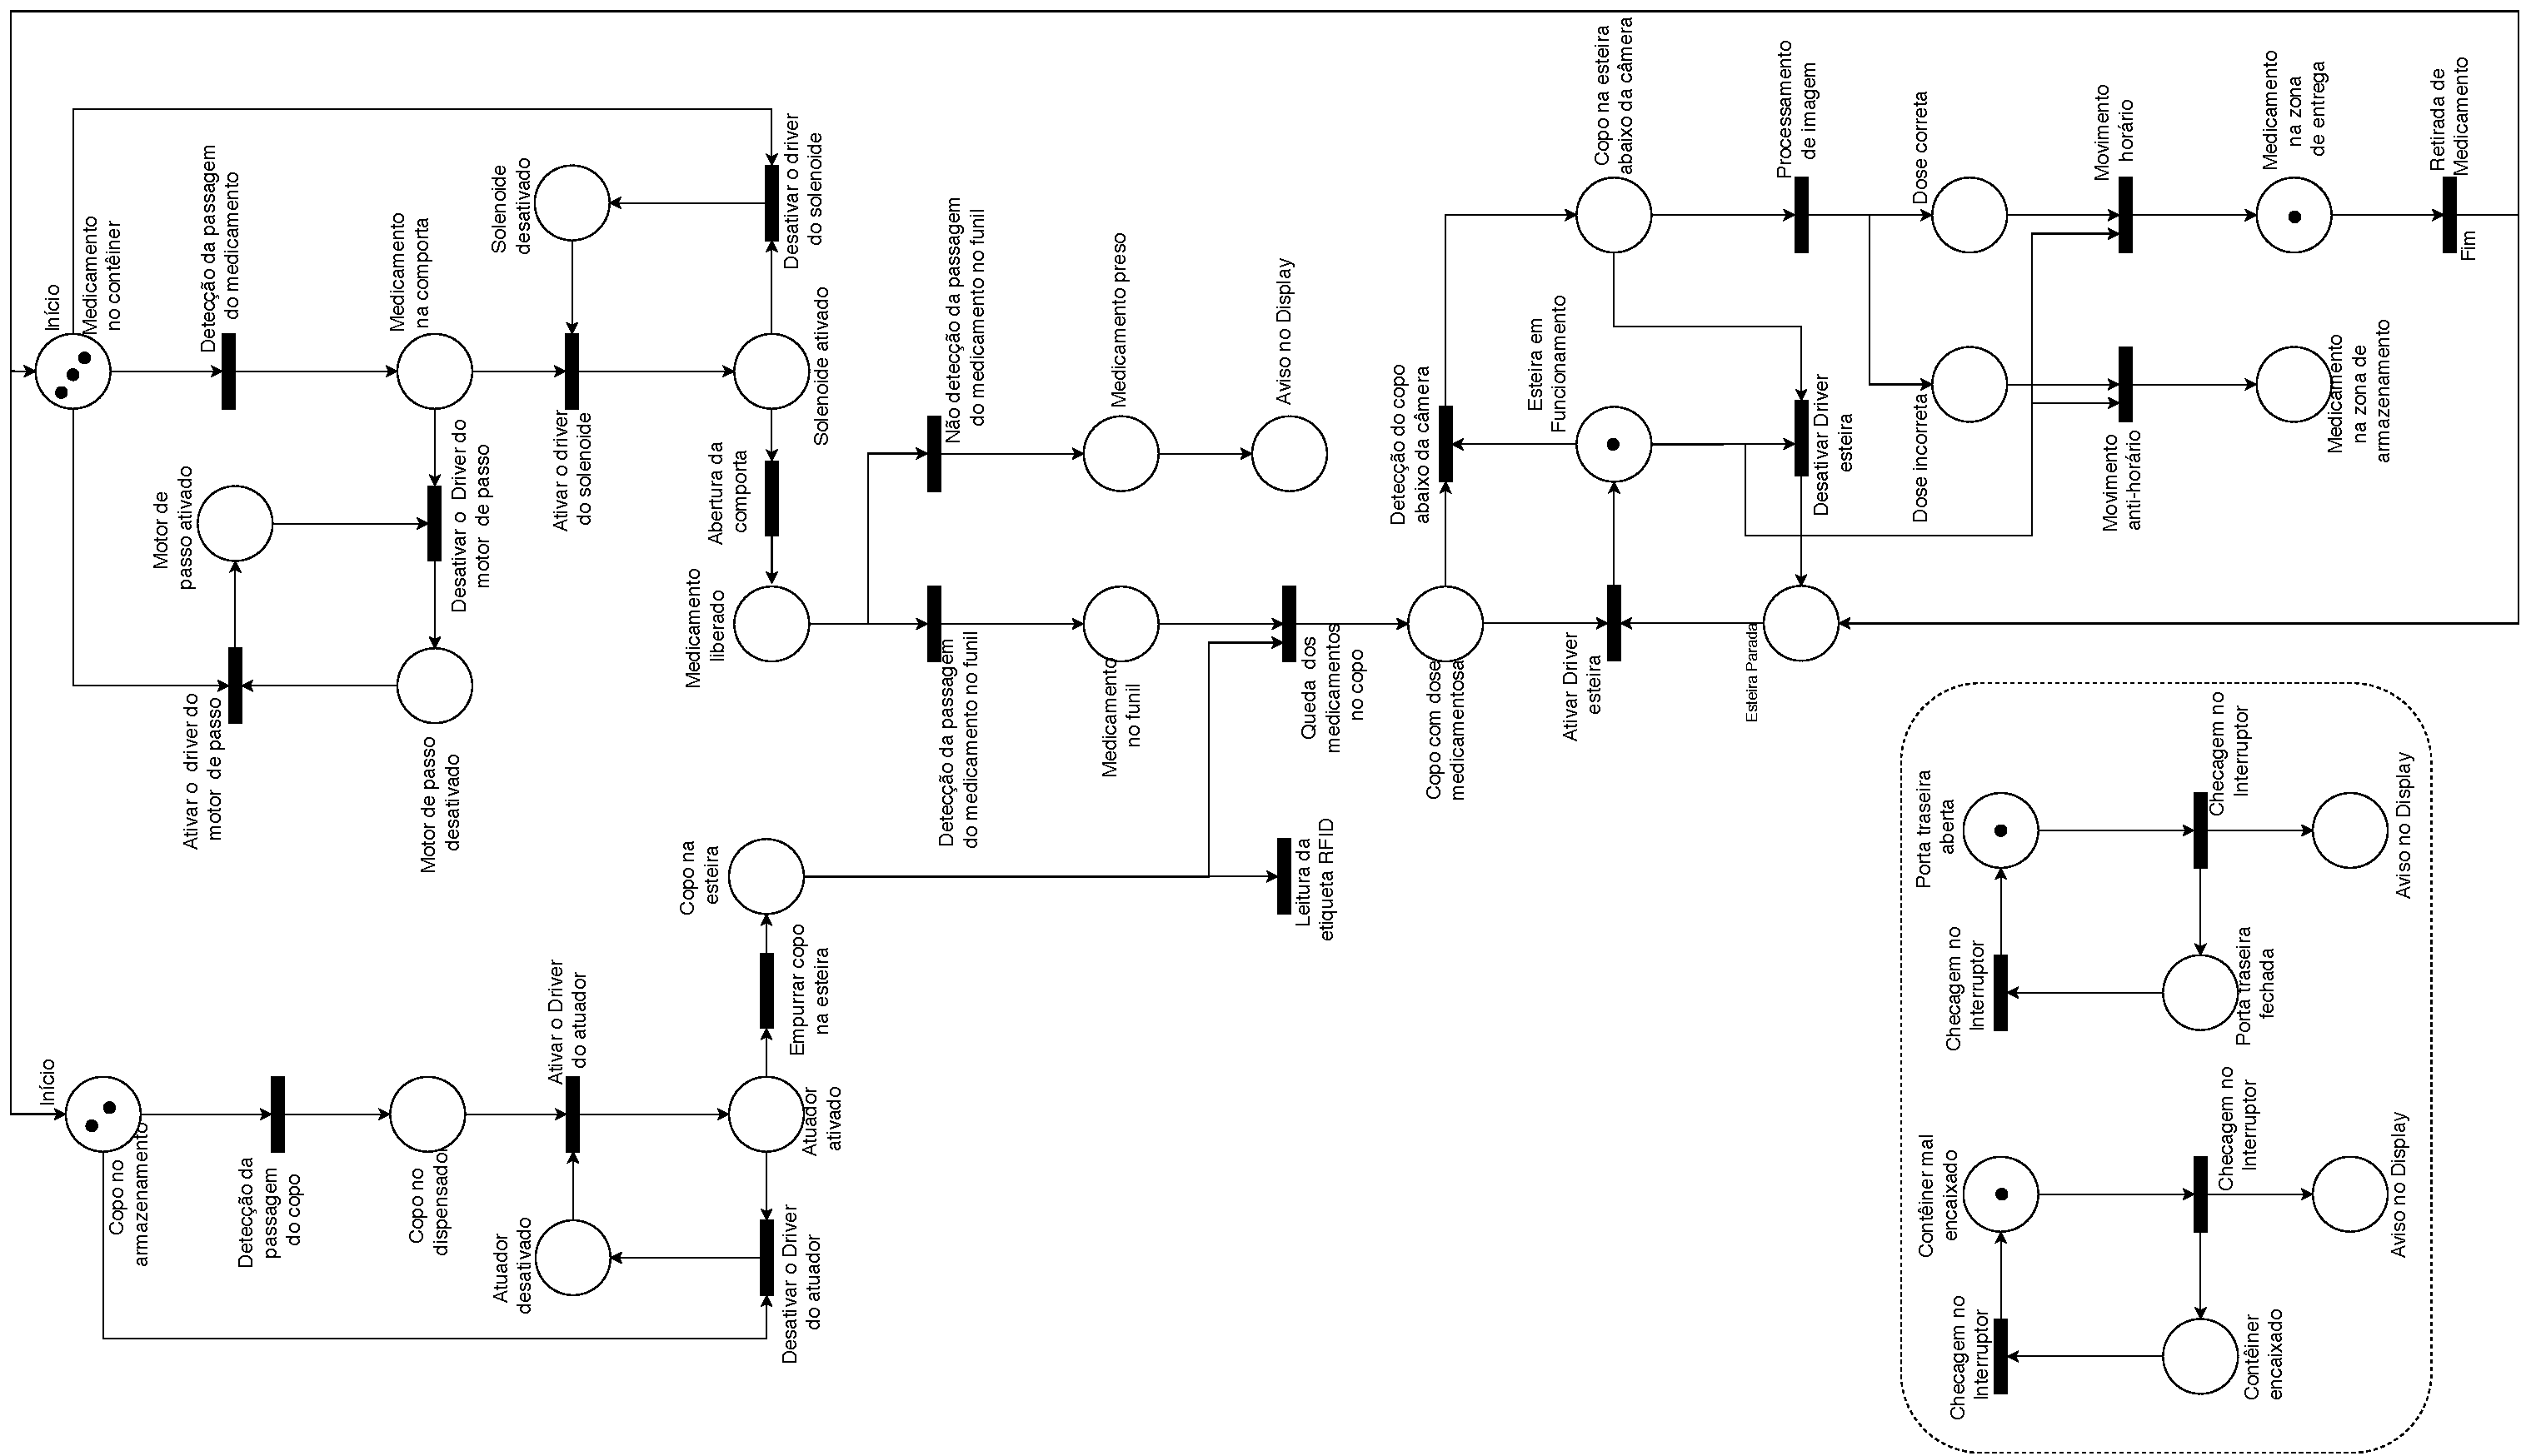
\includegraphics[width=1.4\textwidth, angle = -90]{figuras/eletronica/fluxogramas/petri.pdf}
    \caption{Rede de Petri do Controle eletrônico}
    \label{fig:rede_petri}
\end{figure}

\section{Processamento de Imagens}


\subsection{Separação dos comprimidos}


A primeira etapa para extrair dados da imagem é isolar os comprimidos presentes. Para isso é preciso a conversão da imagem para escala de cinza, facilitando assim na utilização de operações de filtragem na imagem em etapas subsequentes. Para exemplificar a explicação daqui em diante utilizamos uma imagem do banco de dados, original na figura \ref{fig:proOrig}, e aplicando a conversão para escala de cinza temos o resultado na figura \ref{fig:proCinza}.

Em seguida, é necessário a detecção das bordas do comprimido. Como as imagens do banco de dados possuem um fundo padronizado o uso da técnica de limiar é possível. Um resultado possível pode ser observado na figura \ref{fig:proLim}. 

O próximo passo é eliminar resíduos da imagem deixando apenas o contorno do comprimido. Para isso são realizadas operações de abertura e fechamento utilizando elementos estruturantes circulares maiores que o resíduo e menores que o comprimido. Com isso obtemos uma máscara do exemplo utilizado, na figura \ref{fig:proMask}.

Por fim, uma técnica de detecção de objetos conectados é aplicada, a qual consegue separar objetos na imagem por meio de observação da vizinhança na imagem. Aplicando essa técnica nos exemplos temos o resultado nas figuras \ref{fig:proMask1} e \ref{fig:proMask2}.

Com a máscara segmentada é possível separar os comprimidos por meio de uma multiplicação com a imagem original, com isso obtemos as figuras \ref{fig:proPill1} e \ref{fig:proPill2}.

\begin{figure}[H]
        \centering
        \subfloat[][Original]{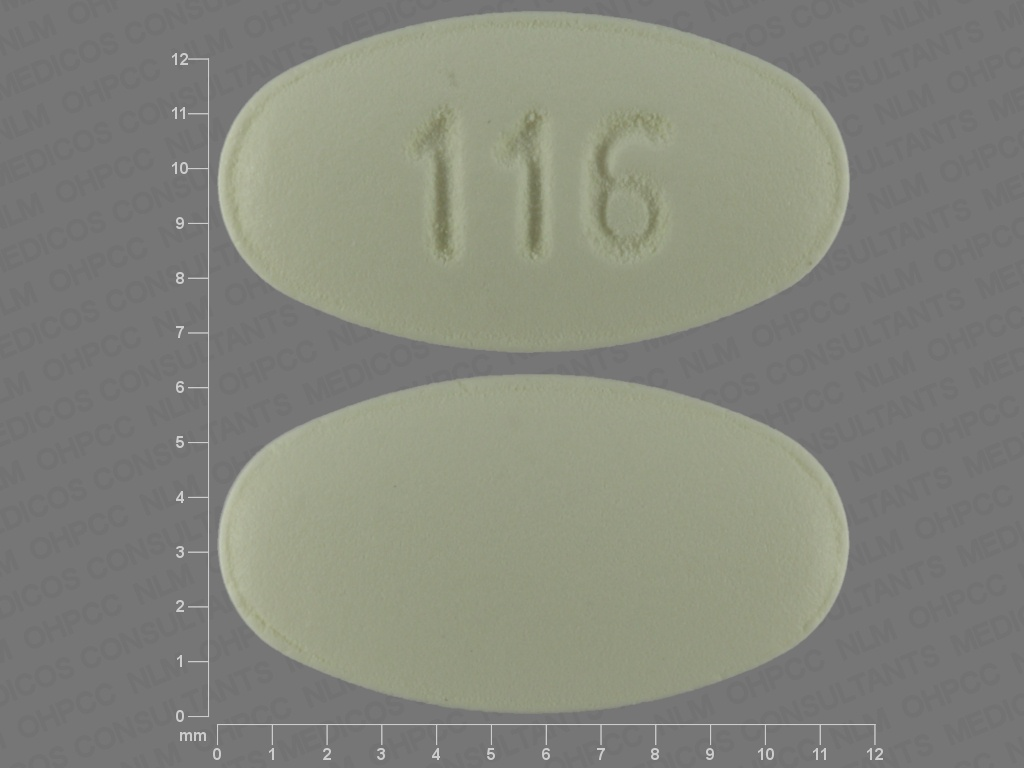
\includegraphics[width=0.3\textwidth]{figuras/processamento/original.jpg}\label{fig:proOrig}}
        %\hspace{0.1\textwidth}
        \subfloat[][Escala de cinza]{
        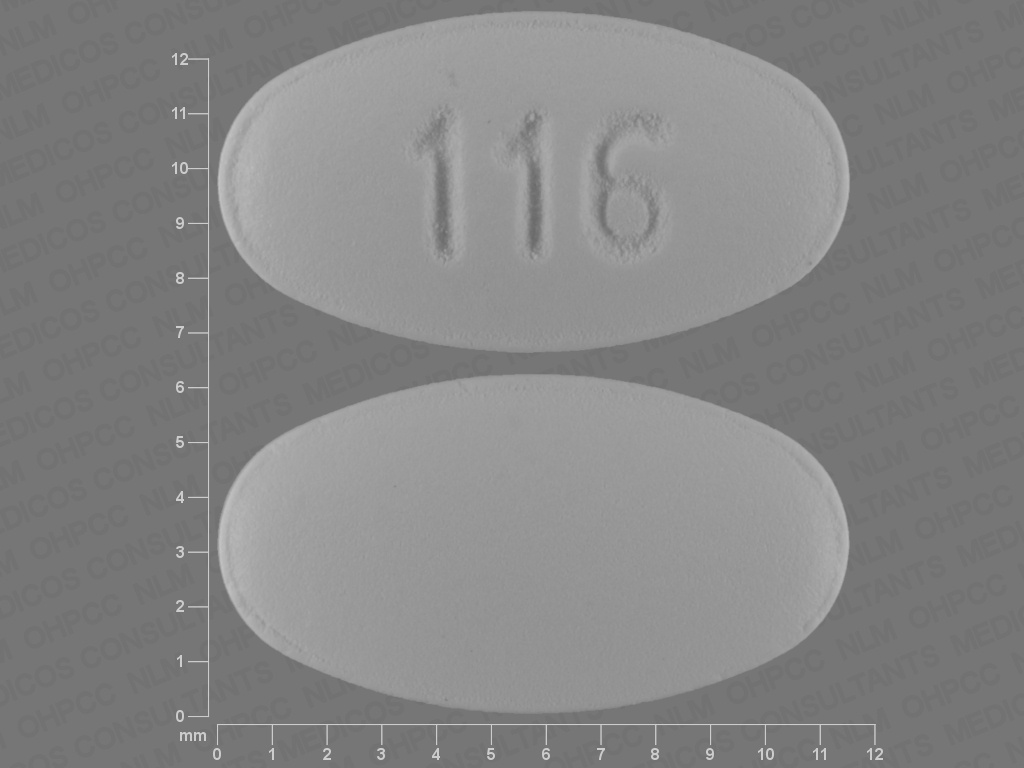
\includegraphics[width=0.3\textwidth]{figuras/processamento/cinza.jpg}\label{fig:proCinza}}
        \subfloat[][Limiar]{
        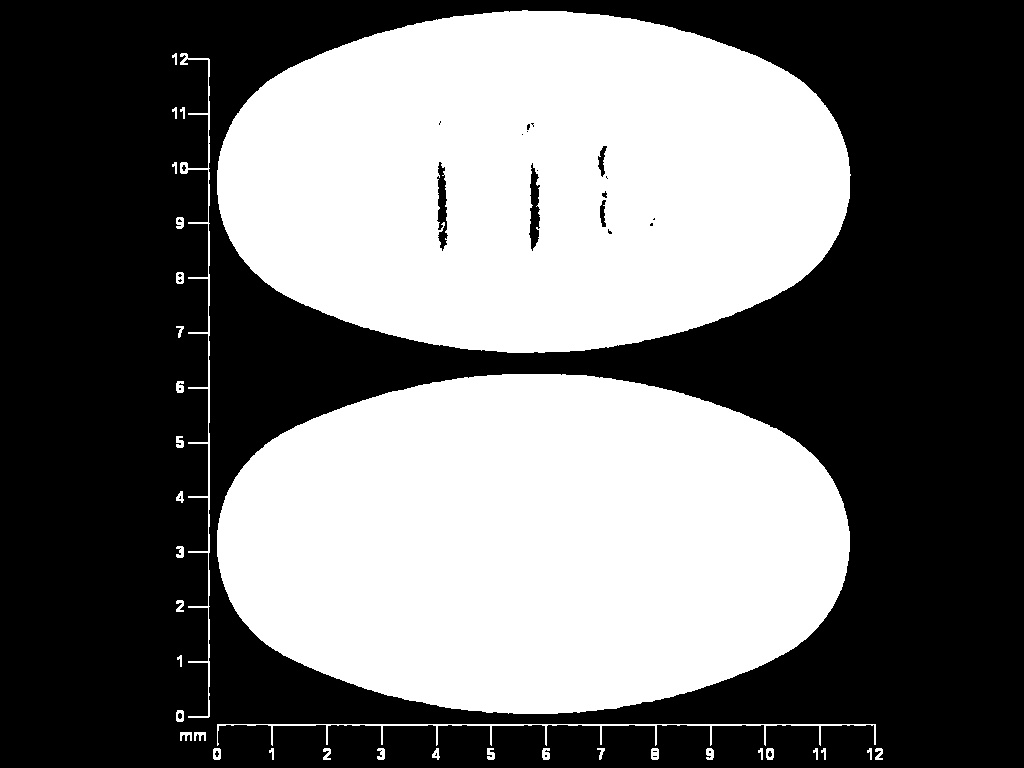
\includegraphics[width=0.3\textwidth]{figuras/processamento/limiar.jpg}\label{fig:proLim}}
        
        \subfloat[][Máscara]{
        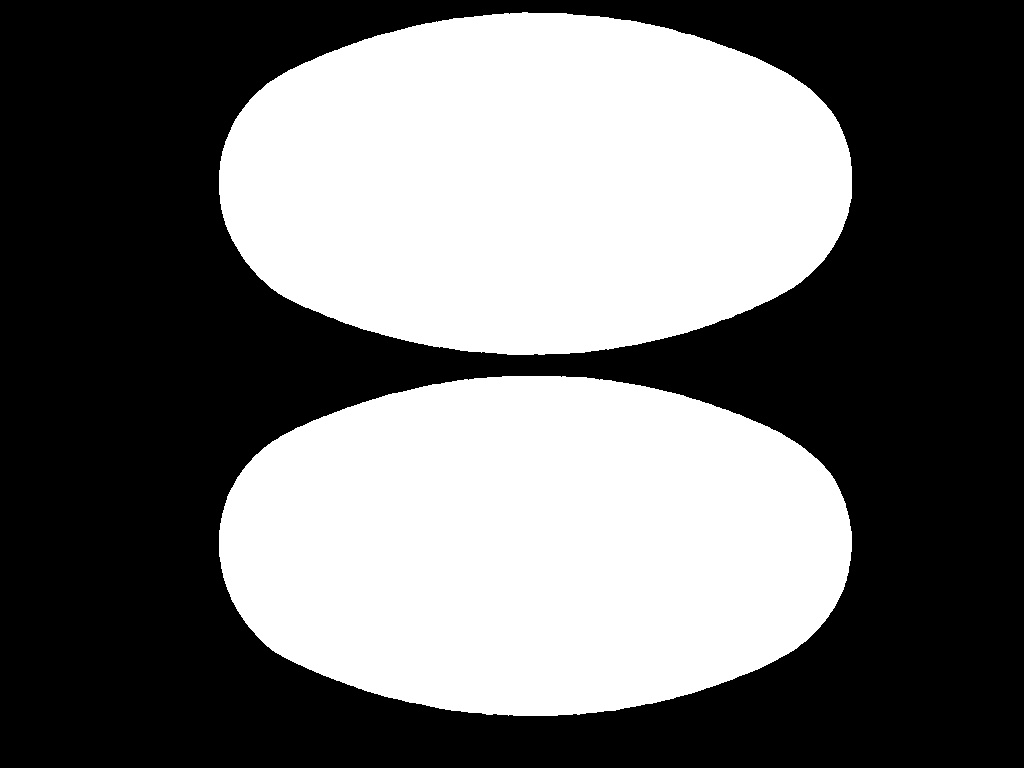
\includegraphics[width=0.3\textwidth]{figuras/processamento/mascara.jpg}\label{fig:proMask}}
        \subfloat[][Objeto 1]{
        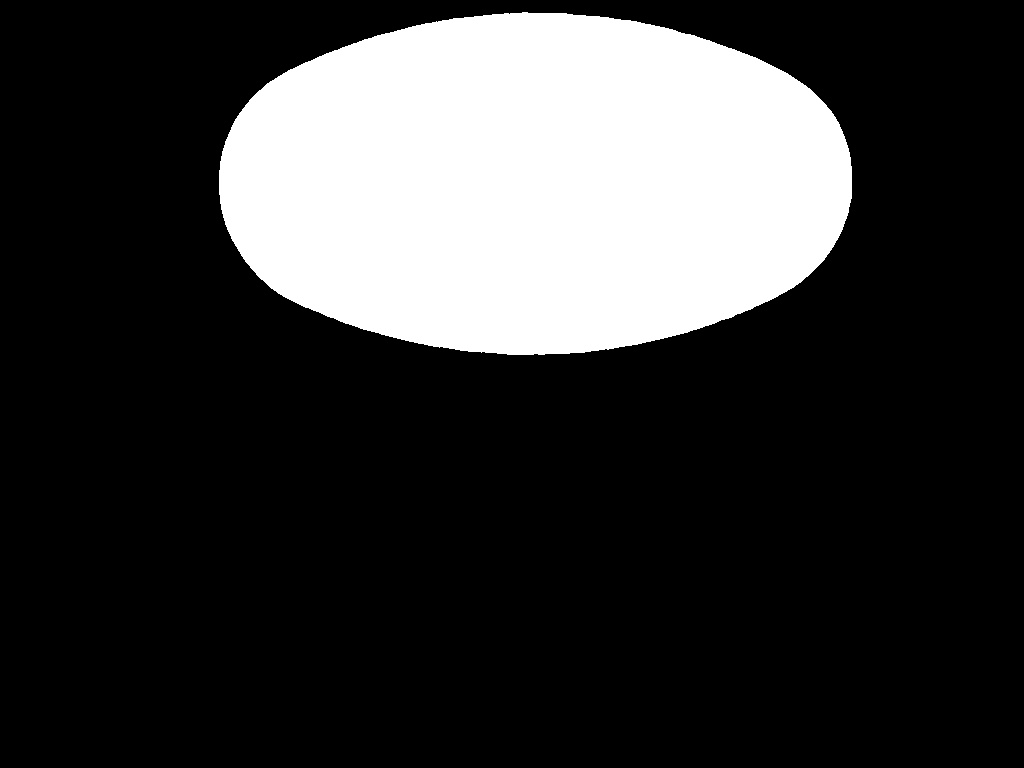
\includegraphics[width=0.3\textwidth]{figuras/processamento/mascara1.jpg}\label{fig:proMask1}}
        \subfloat[][Objeto 2]{
        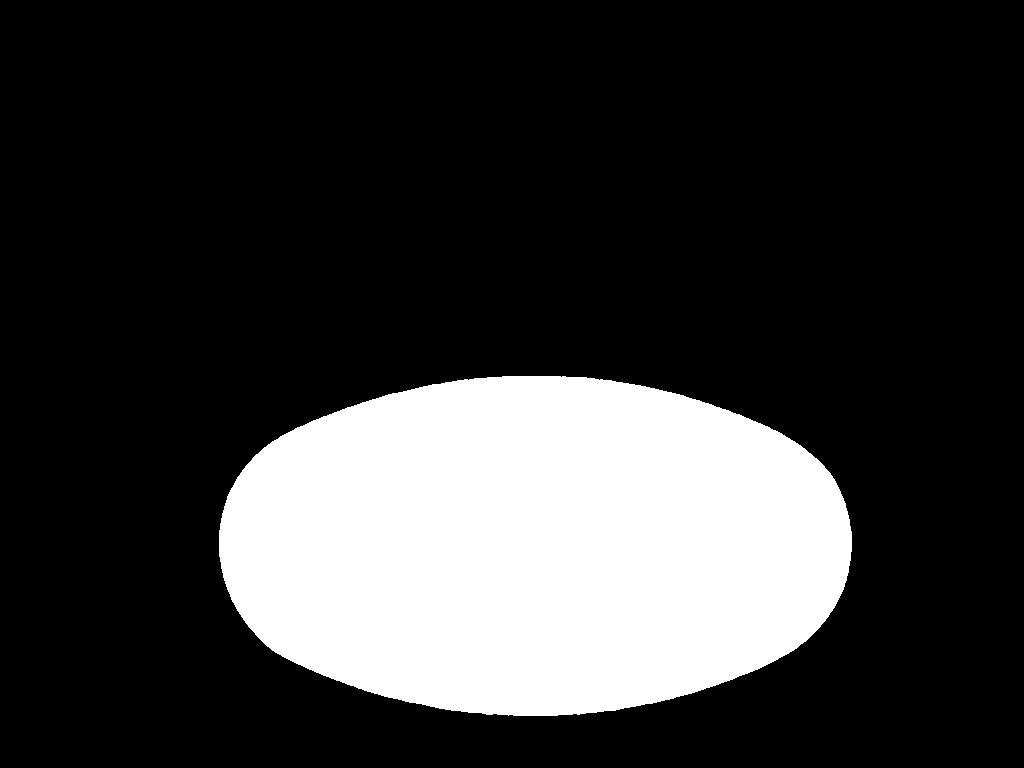
\includegraphics[width=0.3\textwidth]{figuras/processamento/mascara2.jpg}\label{fig:proMask2}}
        
        \subfloat[][Comprimido 1]{
        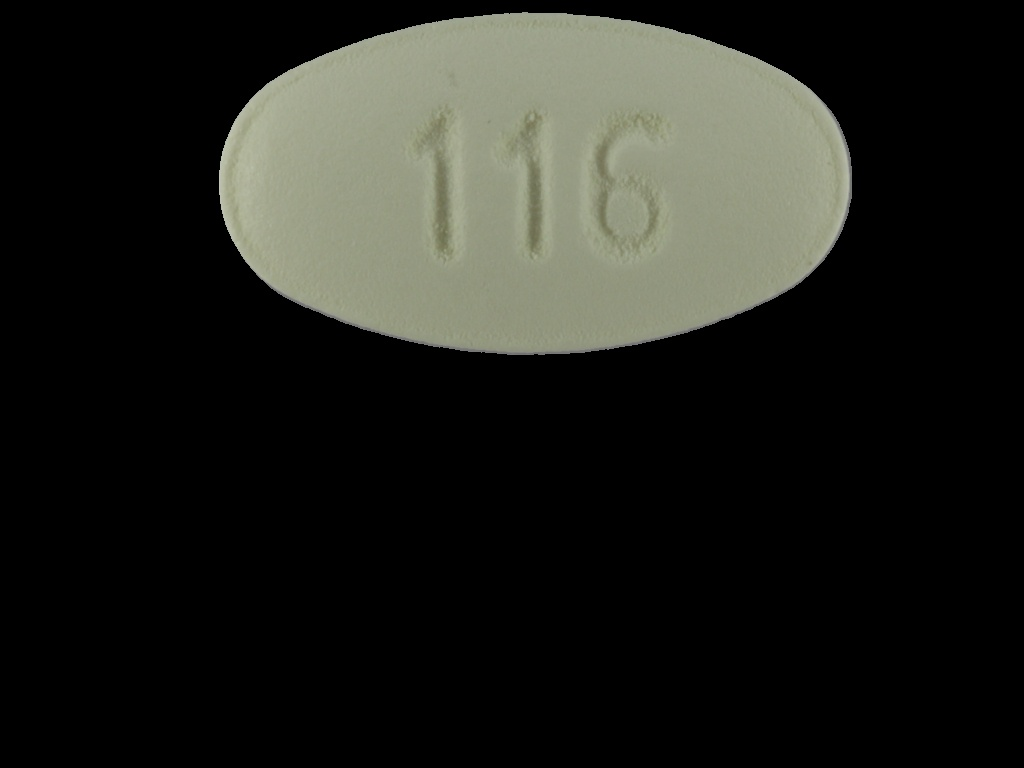
\includegraphics[width=0.3\textwidth]{figuras/processamento/pilula1.jpg}\label{fig:proPill1}}
        \subfloat[][Comprimido 2]{
        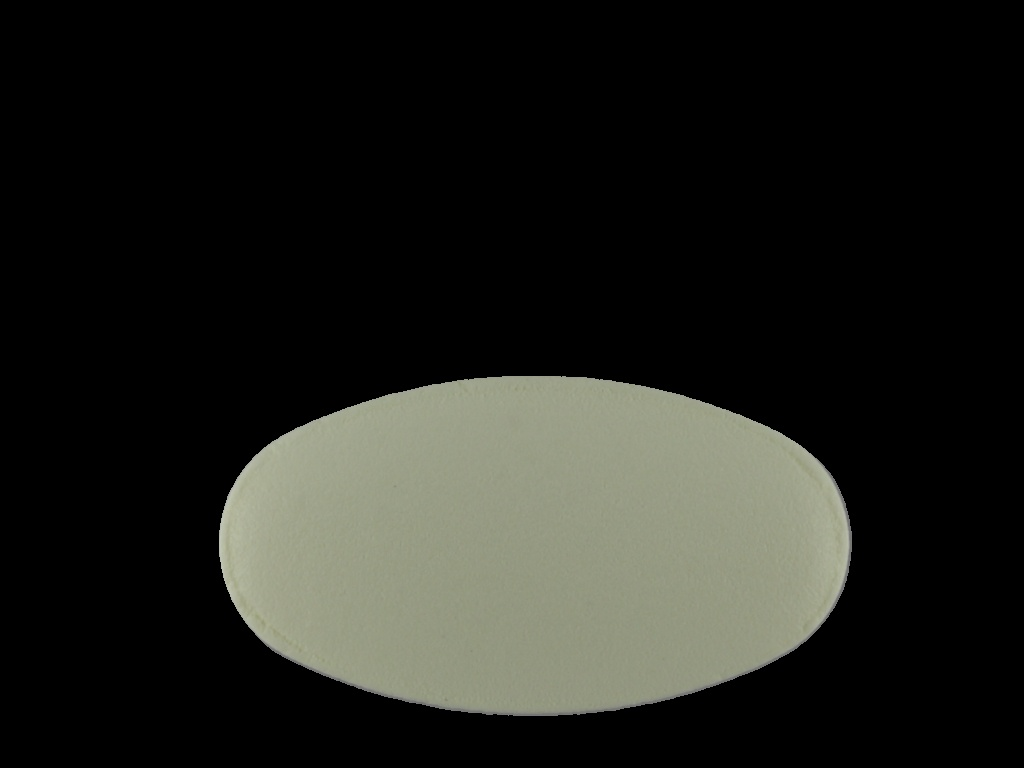
\includegraphics[width=0.3\textwidth]{figuras/processamento/pilula2.jpg}\label{fig:proPill2}}
        
        \caption{Processo de separação}
        \label{fig:proCond}
\end{figure}

\subsection{Extração de características}

Com os comprimidos separados é possível extrair informações que serão utilizadas para classificá-los.

\begin{itemize}
    \item \textbf{Cor}
    
    Para extrair a cor do comprimido será utilizada uma média de cor de toda a região, eliminando possíveis efeitos de sombra presentes. Sendo assim, serão estabelecidos rótulos que corresponderão a uma faixa específica do espectro RGB das imagens.
    
    \newpage
    \item \textbf{Formato}
    
    Para extrair o formato do comprimido será utilizada a técnica de \textit{template matching}. Ela consiste em comparar a imagem com modelos pré-definidos, realizando a correlação da imagem com o \textit{template}, Se essa correlação for próxima de 1 significa que há uma alta probabilidade do formato estar correto. Consequentemente, é possível testar todos os formatos possíveis e identificar qual a maior correlação entre eles.
    
    \item \textbf{Texto estampado}
    
    Para extrair o texto do comprimido é necessário o tratamento da imagem para que os contornos sejam destacados com isso obtemos a figura \ref{fig:propilLim}, porém o objeto de texto ainda possui áreas não conectadas. Para contornar esse problema é utilizado uma abertura na imagem com um objeto estruturante circular pequeno com até 5 pixeis de diâmetro. Assim obtemos como resultado uma melhor definição das letras, mostrado na figura \ref{fig:propilAb}.
    
    Por fim, subtrai-se a máscara do comprimido do resultado anteriormente obtido e, consequentemente, no isolamento do texto a ser processado. O resultado da subtração da máscara pode ser visualizado na figura \ref{fig:propiltext}.
    
    Para interpretar o texto será utilizado o \textbf{Tesseract}, um sistema de reconhecimento óptico de caracteres (OCR) que utiliza uma rede neural treinada para identificar linhas de texto. Para utilização desse sistema é necessário identificar a região de interesse e isolá-la para melhores resultados. Assim obtemos o resultado na figura \ref{fig:propiltextex}, onde é possível observar a região de interesse que possui texto e o valor reconhecido.
    
    \begin{figure}[H]
        \centering
        \subfloat[][Destaque dos contornos]{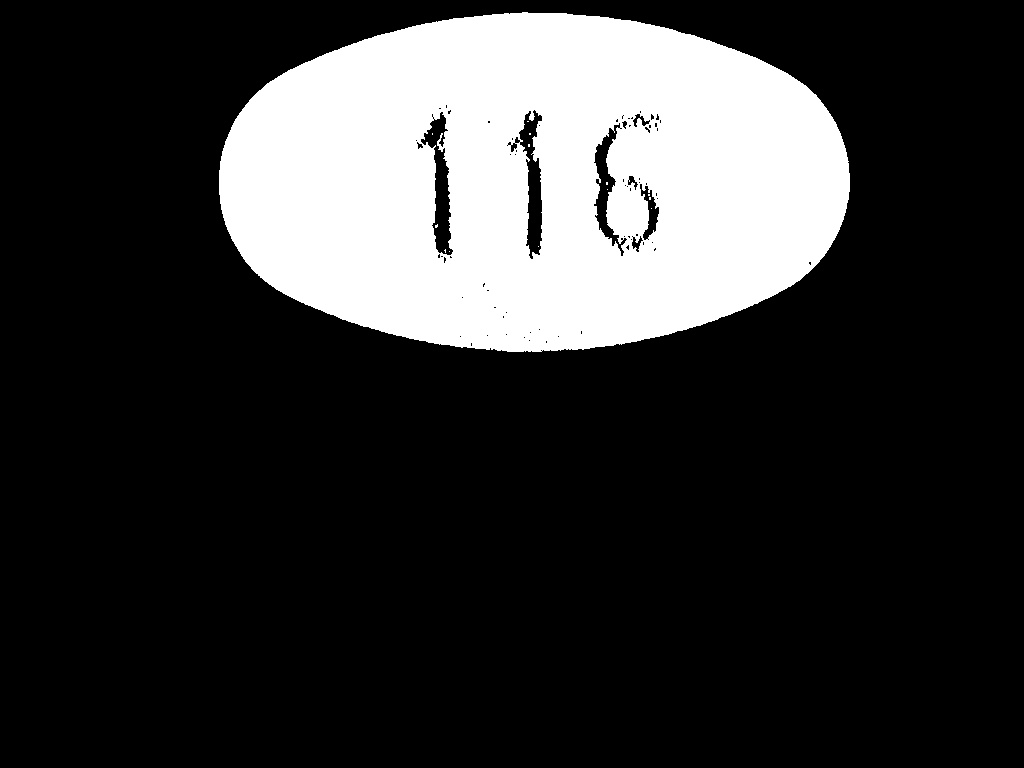
\includegraphics[width=0.3\textwidth]{figuras/processamento/pilulalimiar.jpg}\label{fig:propilLim}}
        \hspace{0.05cm}
        \subfloat[][Conexão das letras]{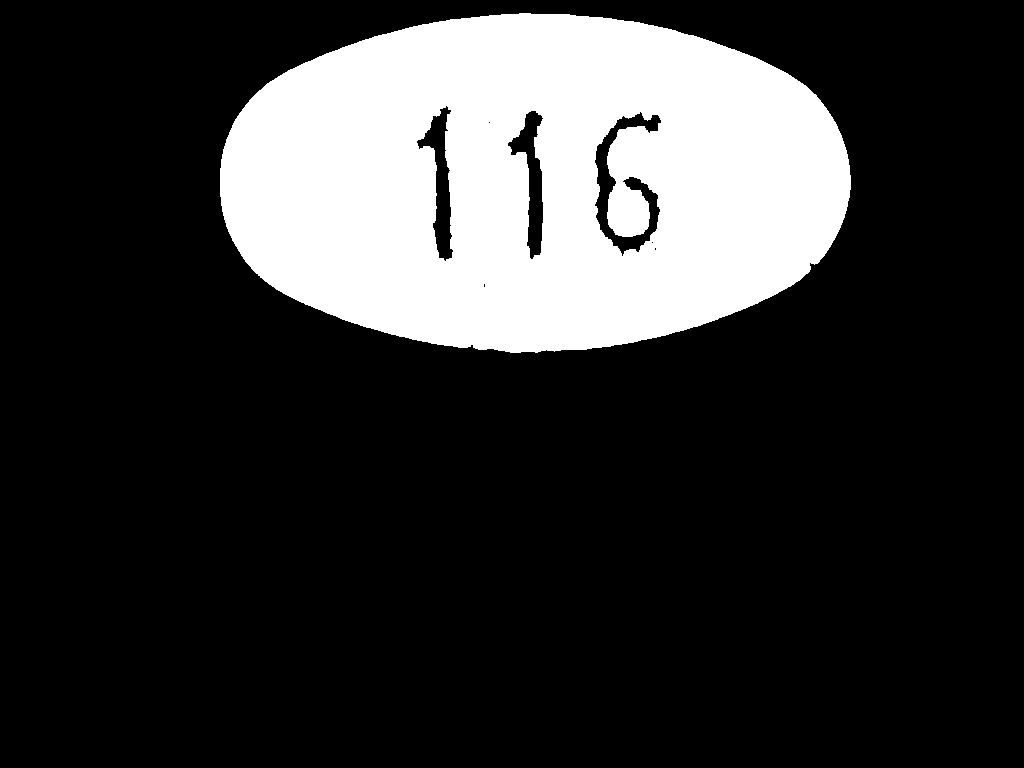
\includegraphics[width=0.3\textwidth]{figuras/processamento/pilulaabertura.jpg}\label{fig:propilAb}}
        \hspace{0.05cm}
        \subfloat[][Texto isolado]{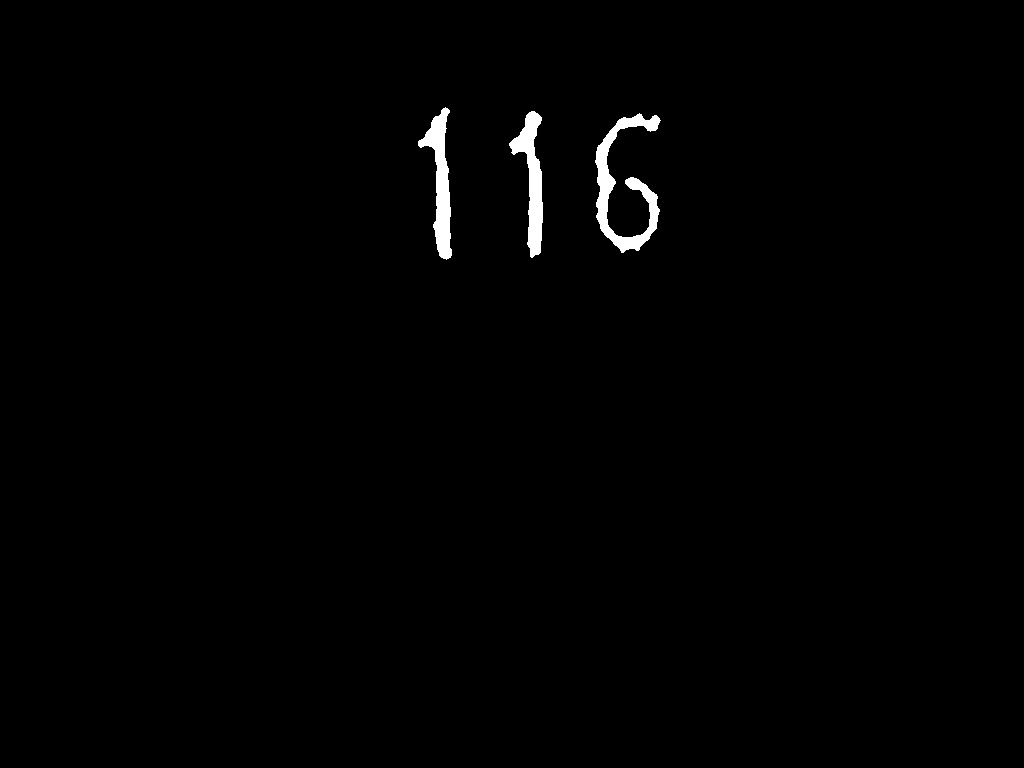
\includegraphics[width=0.3\textwidth]{figuras/processamento/texto.jpg}\label{fig:propiltext}}
        
        \subfloat[][Texto identificado]{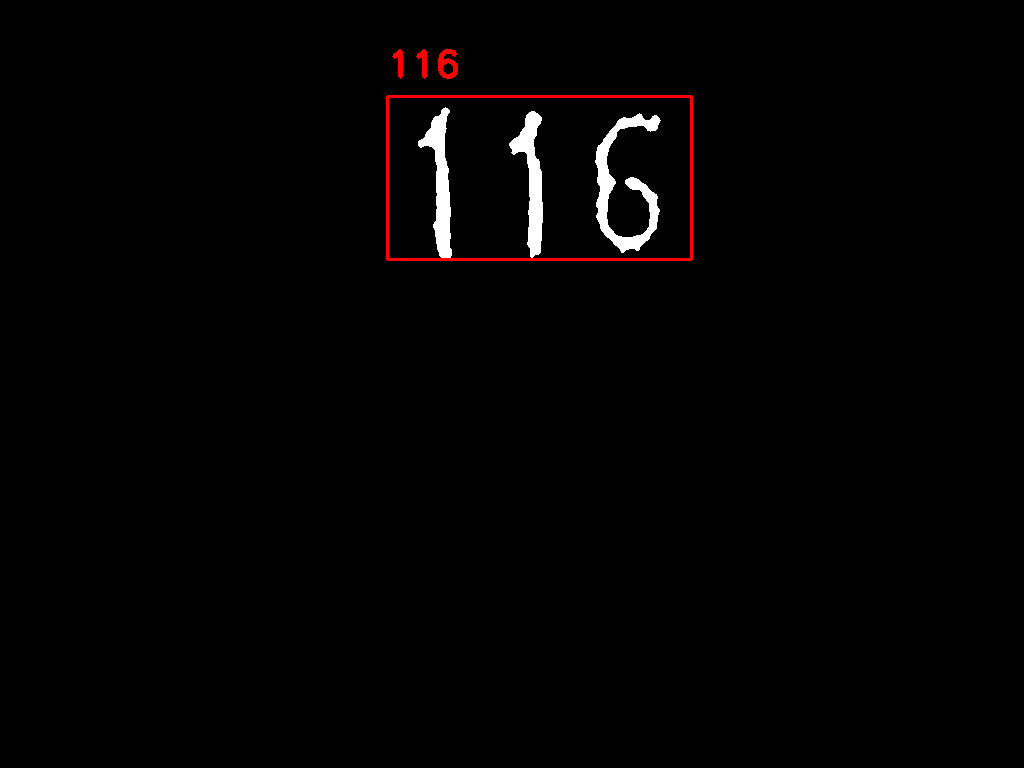
\includegraphics[width=0.4\textwidth]{figuras/processamento/textoExtraido.png}\label{fig:propiltextex}}
        
        
        \caption{Extração de texto}
        \label{fig:proText}
    \end{figure}
\end{itemize}

\subsection{Máquina de Vetores de Suporte (SVM)}

Para conseguir identificar diversos comprimidos nas imagens é necessário o uso de um classificador. Existe diversos tipos de classificos e o escolhido foi a máquina de vetores de suporte (SVM). 

Seu funcionamento se baseia na ideia de gerar uma superfície que separa as classificações por meio das características empregadas. Dessa forma são criados vetores de suporte que separam a área entre classificações, gerando assim os vetores de suporte que deve haver o treinamento da SVM.

Para o treinamento será utilizado um banco de imagens de comprimidos feito pela \textit{National Library of Medicine} que possui 4000 imagens em ambiente controlado e 133000 em imagens amadoras, disponível no  \href{https://www.nlm.nih.gov/databases/download/data_distrib_main.html}{link}. 

O tipo de classificação utilizada será a \textit{yes or no}. Na qual serão criadas SVMs para cada comprimido a ser identificado e ensinando ela para identificar características daquele comprimido.



\section{Plano de Construção}
\label{sec:plano_de_construção}

A construção dos subsistemas da eletrônica foi implementada a partir dos os esquemáticos descritos na seção \ref{sec:esq_conec_sistemas}. Desses esquemáticos podem ser geradas as placas de circuito impresso (PCI), que servem como base para conexão de todos subsistemas e seus componentes da área eletrônica. 

Para o projeto das PCIs foi utilizado o software \textit{Proteus} e tem-se o emprego de placas de fibra de vidro de camada dupla de 1,6 mm de espessura. Em algumas PCIs a camada oposta possui vias passantes para realizar conexões. A largura mínima da trilha é determinada pela espessura do cobre da placa e a corrente máxima que percorre o circuito. Assim, a partir da seleção de uma placa com 3 onças (oz) de espessura do cobre da placa e uma corrente máxima de 3 A é possível determinar a largura da trilha utilizando as fórmulas IPC-2221. Primeiramente, deve-se calcular a área da seção transversal conforme a Eq. \ref{IPC-2221}:

\begin{equation}\label{IPC-2221}
    A = \frac{i \; [\text{A}]}{\left[ k \; [\frac{\text{W}}{\text{m} \cdot ^\circ \text{C}}] \cdot(dT \; [^\circ \text{C}]\textsuperscript{0,44})\right]^{\frac{1}{0,725}} } \quad [\text{mils}^2]
\end{equation}

Em que $A$ é a área da seção transversal, $i$ é a corrente máxima, $dT$ é o aumento da temperatura acima da temperatura ambiente e $k$ é a constante de condutividade térmica, o qual para camadas internas $k=0,024$ enquanto que para camadas externas $k=0,048$ \cite{IPC}. Em seguida a largura é calculada conforme a Eq. \ref{IPC-2221_2}:

\begin{equation}\label{IPC-2221_2}
    L = \frac{A \; [\text{mils}^2]}{\left[(E \; [\text{oz}] \cdot 1,378 \; [\frac{\text{mils}}{\text{oz}}])\right]} \quad [\text{mils}]
\end{equation}

Em que $L$ é a largura da trilha e $E$ é a espessura do cobre na placa. Assim, a partir das Eq. determinou-se que a trilha deve possuir 17,9 mils ou equivalentemente 0,456 mm. Entretanto, para o projeto das PCIs foi adicionado uma folga na largura da trilha, então foi utilizado 25 mils correspondente a 0,635 mm.

Além do mais, as angulações para todas as PCIs foram de 45$^\circ$ e 60$^\circ$ para as vias roteadas, a distância de uma trilha para outra foi de 15 mils (0,381 mm) já que o mínimo é 9 mils (0,229 mm), a distância de uma trilha para um furo é de no mínimo 8 mils (0,200 mm) e a distância entre as inscrições da serigrafia e os \textit{pads} (\textit{SMD}, \textit{Through Hole} e BGA) seja no mínimo de 5 mil (0,127mm).

Ademais, foram utilizados conectores \textit{Molex} KK e uma legenda em cada conector da PCI para evitar a conexão errada de algum componente, tanto em tipo quanto na orientação do cabo. As figuras no apêndice \ref{app:PCB} mostram os \textit{layouts} para as placas fabricadas. Em todos os casos foram utilizadas zonas preenchidas de \textit{Ground} (GND) na camada de cobre.

Para uma descrição visual da conexão entre os componentes e as PCIs estão descritos no manual de montagem, apêndice \ref{manual_montagem}.

\subsection{Central de Controle}

A PCI do sistema central, Fig. \ref{fig:PCB_central}, é a que se conecta com a \textit{Raspberry Pi} 4. Essa conexão é feita usando um cabo IDE entre a barra de pinos macho 2x20 dessa PCI e o \textit{GPIO} da \textit{Raspberry Pi} 4. As conexões realizadas na PCI são:

\begin{itemize}
    \item Fonte de alimentação 5 V/8 A: Cabo com conector \textit{Molex} KK de 2 pinos fêmea/fêmea;
    \item LCD 240x320: Cabo com conector \textit{Molex} KK de 8 pinos fêmea/fêmea;
    \item Quatro PCIs que contêm os microcontroladores: 4 Cabos com conector \textit{Molex} KK de 4 fêmea/fêmea;
    \item Sensor Temperatura e Umidade HTU21D: Cabo com conector \textit{Molex} KK de 4 pinos fêmea/fêmea;
    \item Sensor RFID PN532: Cabo com conector \textit{Molex} KK de 4 pinos;
    \item Sensor de Biometria: Cabo com conector \textit{Molex} KK de 6 pinos;
    \item Porta USB tipo A: Cabo com USB tipo A macho e USB tipo C macho
\end{itemize}


Na \textit{Raspberry Pi} 4 são conectados os seguintes componentes:

\begin{itemize}
    \item[]
    \begin{itemize}
        \item Cabo \textit{flat} de 15 canais com 300 mm no \textit{socket} ZIF. Outra ponta dessa cabo é conectado na câmera OV5647;
        \item Cabo USB tipo C vindo da PCI na porta de alimentação;
        \item \textit{SD Card} de 32GBs com a imagem do OS Ubuntu 18.04.03 modificado para o projeto no respectivo \textit{socket}.
    \end{itemize}
\end{itemize}


\subsection{Módulo de Medição}\label{sec:construcao_modulo_medicao}

Para o módulo de medição são utilizados duas placas PCI (PIC16 1 e PIC16 2), representação esquemática nos esquemáticos 2 (Fig. \ref{fig:esquematico_2}) e 3 (Fig. \ref{fig:esquematico_3}).

Na PCI especificada como PI16 1, Fig. \ref{fig:PCB_micro1}, ocorre as seguintes conexões:

\begin{itemize}
    \item[]
    \begin{itemize}
    \item \textbf{Conexão com a PCI central:} Cabo com conexão \textit{Molex} KK de 4 pinos fêmea/fêmea que foi conectado no conector de legenda PIC16 1 na PCI central.
    \item \textbf{Conexão dos 30 Sensores de Barreira:} 30 Cabos com conexão \textit{Molex} KK de 2 pinos fêmea/fêmea com a outra ponta conectada as 30 PCIs representadas na Fig. \ref{fig:PCB_barreira}.
\end{itemize}
\end{itemize}

Na PCI do sensor de barreira, Fig. \ref{fig:PCB_barreira}, além de ser conectado o cabo vindo a PCI PIC16, devemos utilizar 2 cabos adicionais com 2 terminais cada para conectar o PT333-3B e IR333 para cada sensor.

Na PCI especificada como PI16 2, Fig. \ref{fig:PCB_micro2}, ocorre as seguintes conexões:

\begin{itemize}
    \item[]
    \begin{itemize}
    \item \textbf{Conexão com a PCI central:} Cabo com conexão \textit{Molex} KK de 4 pinos fêmea/fêmea que foi conectado no conector de legenda PIC16 2 na PCI central.
    \item \textbf{Conexão das 33 Chaves \textit{Micro Switch}:} 33 Cabos com conexão \textit{Molex} KK de 2 pinos fêmea/fêmea com a outra ponta conectada as chaves no terminal Comum e Normal Fechado (Pino 1 e Pino 2).
    \item \textbf{Teclado:} Cabo com conexão \textit{Molex} KK de 3 pinos fêmea/fêmea
\end{itemize}
\end{itemize}

\subsection{Módulo de Acionamento dos Atuadores}

Para o módulo de acionamento dos atuadores são utilizados duas placas PCI (PIC16 3 e PIC16 4), representação esquemática nos esquemáticos 4 (Fig. \ref{fig:esquematico_4}) e 5 (Fig. \ref{fig:esquematico_5}).

Na PCI especificada como PI16 3, Fig. \ref{fig:PCB_micro3}, ocorre as seguintes conexões:

\begin{itemize}
    \item[]
    \begin{itemize}
    \item \textbf{Conexão com a PCI central:} Cabo com conexão \textit{Molex} KK de 4 pinos fêmea/fêmea que foi conectado no conector de legenda PIC16 3 na PCI central.
    \item \textbf{Conexão de 32 solenoides (\textit{driver} IRF520N):} 32 Cabos com conexão \textit{Molex} KK de 2 pinos fêmea/fêmea com a outra ponta conectada aos pinos de sinal e GND do \textit{driver} IRF520N.
    \item \textbf{Conexão com Atuador Linear (\textit{driver} IRF520N):} Um cabo com conexão \textit{Molex} KK de 2 pinos fêmea/fêmea com a outra ponta conectada aos pinos de sinal e GND do \textit{driver} IRF520N.
\end{itemize}
\end{itemize}

De fábrica os cabos da solenoide vem com um conector molex KK não compatível com a conexão do \textit{driver}. Sendo assim, é necessário sua remoção e desencapamento dos fios vermelho e preto da solenoide. Em seguida inserimos os fios no borne de duas entradas do \textit{driver} IRF520N (Vermelho no V+ e Preto no V-).

Para a conexão do atuador com o \textit{driver} IRF520 é inserido os fios do atuador no borne (Positivo em V+ e Negativo em V-).


Na PCI especificada como PI16 4, Fig. \ref{fig:PCB_micro4}, ocorre as seguintes conexões:

\begin{itemize}
    \item[]
    \begin{itemize}
    \item \textbf{Conexão com a PCI central:} Cabo com conexão \textit{Molex} KK de 4 pinos fêmea/fêmea que foi conectado no conector de legenda PIC16 4 na PCI central.
    \item \textbf{Conexão dos 5 \textit{drivers} A4988:} Cabo com conexão \textit{Molex} de 9 pinos fêmea / pinos fêmea 
    \item \textbf{\textit{Driver} L298:} Cabo com conexão \textit{Molex} de 3 pinos fêmea / pinos fêmea
\end{itemize}
\end{itemize}

Para conexão do motor de passo (NEMA 13) com \textit{driver} A4988 conectamos os fios na seguinte ordem:

\begin{itemize}
    \item[]
    \begin{itemize}
        \item Fio vermelho do motor no terminal 2B
        \item Fio azul do motor no terminal 2A
        \item Fio verde do motor no terminal 1B
        \item Fio preto do motor no terminal 1A
    \end{itemize}
\end{itemize}

Para conexão do motor DC no \textit{driver} L298 inserimos os 2 fios (motor) no borne de 2 entradas para o motor A (ao lado do borne de 3 que se conecta a alimentação para o \textit{driver}).


\section{Firmware Embarcado}% ?Mudar nome da secao
Após a construção física das conexões do sistema, deve-se desenvolver o \textit{Firmware} do sistema embarcado.Pode-se dividir a implementação em duas partes. A primeira se refere aos módulos de medição e de acionamento dos atuadores, que serão programados em linguagem C por meio do compilador \textbf{CCS C} para microcontroladores da família \textit{PIC}.

A segunda se relaciona à central de controle, a qual será programada em linguagem \textit{Python 3}. Todos os códigos desenvolvidos podem ser acessados por meio do repositório do link: \href{https://github.com/PillWatcher/pillwatcher-embarcado}{PillWatcher-Embarcado}

\subsection{Protocolo I$^2$C}

O desenvolvimento de uma lógica de leitura e escrita do protocolo é necessário nos microcontroladores, o primeiro passo é ajustar o microcontrolador para o modo escravo por meio da diretiva \textbf{\#use i2c(SLAVE)}. A próxima etapa é ler o estado de comunicação por meio da função \textbf{int8 2c\_isr\_state()}, o estado retornado representa a operação que será realizada, estados menores que \textbf{0x80} representam endereços e dados, enquanto valores iguais ou superiores a \textbf{0x80} representam a requisição de dados para o microcontrolador.

Para ler os bytes recebidos é utilizada a função \textbf{int8 i2c\_read()} que retorna o byte presente no \textit{buffer}. Para enviar um byte de resposta é utilizada a função \textbf{int1 i2c\_write(unsigned int8 data)} que escreve no barramento I$^2$C.

\subsection{Módulo de Medição}

\begin{itemize}
    \item Sensores de barreira
    
    O \textit{firmware} responsável pelos sensores de barreira possui em sua memória uma tabela para a seleção do sensor que será lido. Nessa tabela estão presentes seis valores lógicos para a seleção no multiplexador, sendo três valores para seleção da porta e três valores para seleção do multiplexador ativo. O último valor na tabela se refere ao pino de entrada no microcontrolador para leitura dos sinais. Dessa forma estão posicionados 24 sensores de barreira nos multiplexadores e 6 diretamente ligados ao microcontrolador.
    
    Para utilização do protocolo I$^2$C foi escolhido o endereço de comunicação \textbf{0xA0}. O valor recebido representa o endereço do sensor na tabela, dessa forma os pinos são condicionados e o estado do sensor é enviado em retorno.
    
    \item Chave e teclado
    
    O \textit{firmware} segue a mesma lógica dos sensores de barreira, entretanto possui 32 chaves conectadas em 4 multiplexadores, dessa forma a tabela possui 7 valores lógicos de seleção do multiplexador, há dois sensores conectados diretamente ao microcontrolador, uma chave e o teclado.
    
    Para ler os dados do teclado é utilizado o conversor A/D presente no microcontrolador, utilizando como referência a tensão de alimentação. Com isso tem-se cinco faixas de tensão estipuladas para os parâmetros do teclado. O valor obtido da conversão é comparado com essas faixas e o botão pressionado é retornado por meio do protocolo I$^2$C com bytes com valores de 1 a 5.
    
    O endereço escolhido para comunicação I$^2$C foi \textbf{0xA2}, os valores enviados representam o sensor requerido. Com o valor 0 representado os botões e valores de 1 a 33 representando as chaves. 
\end{itemize}

\subsection{Módulo de Acionamento dos Atuadores}
\begin{itemize}
    \item Solenoides
    
    Como no módulo de medição, o \textit{firmware} possui uma tabela com valores lógicos para seleção do solenoide requerido, entretanto é utilizado o modo demultiplexador, modificando o nível lógico da saída pra acionar o \textit{driver} do solenoide requerido. Os 32 solenoides são posicionados em 4 demultiplexadores, o atuador linear é conectado diretamente ao microcontrolador.
    
    A comunicação I$^2$C possui o endereço escolhido de \textbf{0xA4}, os valores recebidos para o acionamento são o número do solenoide na memória, e o estado de atuação ligado ou desligado, o valor 0 do endereço se refere ao atuador linear, os valores 1 a 32 representam os solenoides. O estado de atuação é estruturado em 0 para desligado e 1 para ligado.  
    
    \item Motores
    
    O \textit{firmware} responsável pelos motores possui uma tabela com os pinos de ativação de cada motor de passo. todos os pinos de controle são conectados ao microcontrolador.
    
    Para a comunicação I$^2$C o endereço escolhido foi \textbf{0xA6}, os valores recebidos são o atuador que será acionado, 0 para o motor DC e 1 a 5 para motores de passo, em seguida é recebida a direção de rotação, 0 para anti-horário, 1 para horário. Então é recebido o número de passos que o motor dará ou a ativação do motor DC, o último valor recebido representa o período dos pulsos enviados ao \textit{driver} dos motores de passo controlando a velocidade ou o \textit{Duty cycle} do PWM para o motor DC, variando de 0 a 255.
\end{itemize}

\subsection{Central de controle}
A central de controle será programada em \textit{Python 3} por meio da utilização de bibliotecas de comunicação com os sensores, atuadores e \textit{back-end}
\begin{itemize}
    \item \textbf{PN532}
    
    Para comunicação com o sensor RFID PN532 será utilizada a biblioteca py532lib, por meio dela é possível ler \textit{Tags} NFC utilizando os métodos na classe \textbf{Pn532\_i2c} que se comunica pelo protocolo I$^2$C. O endereço utilizado pelo sensor é o \textbf{0x24}. 
    
    \item \textbf{HTU21D}
    
    Será utilizada a biblioteca \textbf{Adafruit\_HTU21D} para a comunicação do sensor, o endereço I$^2$C empregado é \textbf{0x40}. Para capturar a temperatura e umidade é necessário o uso dos métodos  \textbf{read\_temperature} e \textbf{read\_humidity} presentes na classe HTU21D.
    
    \item \textbf{DY50}
    
    O sensor DY50 realiza todo o processamento de digitais internamente em sua memória, para enviar comandos é utilizado o protocolo UART, para isso a biblioteca \textbf{python-fingerprint} será utilizada. O primeiro passo é abrir comunicação serial por meio da classe \textbf{PyFingerprint} com ela é possível cadastrar e identificar digitais armazenadas na memória do dispositivo.
    
    \item \textbf{OV5647}
    
    Para comunicação com a câmera será utilizada a biblioteca \textbf{picamera} que torna possível a aquisição de imagens por meio da classe \textbf{PiCamera} que possui o método de captura.
    
    \item \textbf{ILI9341}
    
    Para a comunicação por SPI com o visor ILI9341 será utilizada a biblioteca \textbf{Adafruit\_ILI9341} por meio dela é possível desenhar formas do display e apresentar imagens utilizando a classe ILI9341.
    
    \item \textbf{Rotina de seleção de medicamento}
    
    Após receber o endereço do contêiner, a chave de encaixe correspondente é lida para checar a presença do contêiner selecionado,o motor de passo correspondente é acionado,aciona-se o solenoide correspondente e lê-se o sensor de barreira presente na saída do contêiner até a detecção da passagem do medicamento. O último passo é a detecção da passagem do medicamento pelo funil por meio da leitura do sensor de barreira presente no funil. A rotina só é acionada se houver um copo abaixo do seletor.
    
    \item \textbf{Rotina de posicionamento do copo no seletor de medicamentos}
    
    o sistema aciona o atuador linear para o dispensador de copos, em seguida o motor da esteira é acionado e o sensor de barreira presente na posição de é lido em  até a detecção do copo, feita a detecção, o motor da esteira é desligado. Em seguida é feita a tentativa de leitura da TAG RFID presente no copo, se a leitura for adquirida, a posição do copo é confirmada.
    
    \item \textbf{Rotina de posicionamento do copo na saída ou reciclagem}
    
    O sistema aciona a esteira para a direção da saída ou reciclagem, o sensor de barreira respectivo é lido até a detecção da passagem do copo, em seguida o motor da esteira é desligado.
    
    \item \textbf{Rotina de detecção de fechamento de portas e encaixe de contêineres}
    
    Uma varredura do estado de todas as chaves de encaixe e das portas é feita a cada 15 minutos, para detectar mal contato de contêineres e mal fechamento de portas.
    
    \item \textbf{Rotina de preparação de dose medicamentosa}
    
    O banco de dados de medicamentos é checado a cada 1 minuto em busca de horários de doses medicamentosas com 5 minutos adiantados, quando há uma dose programada, as rotinas de posicionamento do copo e seleção de medicamento são feitas para cada medicamento até completar a dose, em seguida é realizada a rotina de verificação dos medicamentos, se a verificação for positiva, então o copo é posicionado na saída e a rotina de identificação de digital é iniciada.
    Também há a possibilidade de receber comandos para preparação dos medicamentos pelo protocolo MQTT por meio do tópico \textit{\textbf{apply-medication}}, o que substitui a checagem do banco de dados local.
    
    \item \textbf{Rotina de biometria}
    
    A rotina espera uma digital ser identificada no sensor e aciona a trava elétrica da porta especificada para abri-la, com isso retorna o identificador do enfermeiro e aciona a rotina de fila de doses medicamentosas se a porta especificada for a de saída.
    
    \item \textbf{Rotina de fila de doses medicamentosas}
    
    A rotina lê o sensor de barreira na porta de saída, quando uma dose medicamentosa é retirada, se houverem mais doses preparadas na fila, a esteira é acionada 
    até a detecção do próximo copo, e uma mensagem de retorno é enviada ao \textit{broker} MQTT por meio do tópico \textit{\textbf{medication-response}}. O processo se repete até a fila se esgotar.
    
    \item \textbf{Rotina de atualização de dados de doses medicamentosas} 
    
    Diariamente o sistema realiza uma requisição de dados HTTP ao \textit{back-end} para obtenção de dados atualizados, após uma conferência da integridade dos dados recebidos, o banco de dados local é trocado pelo atualizado.
    
    \item \textbf{Rotina de cadastro de enfermeiro}
    
    Por meio do protocolo MQTT o sistema escuta o tópico \textbf{\textit{create-nurse}} presente no \textit{broker} do \textit{back-end} quando uma nova mensagem é recebida, a máquina aciona o visor com uma mensagem para cadastro do enfermeiro recebido.
    
    Assim o leitor de digitais é acionado para cadastro, quando a digital é cadastrada com sucesso, uma mensagem de sucesso é escrita na tela, quando há erro no cadastro, uma mensagem de erro é escrita e o sensor é acionado novamente para cadastro.
    
    \item \textbf{Rotina de abastecimento de medicamentos}
    
    Por meio do protocolo MQTT são escutados os tópicos \textit{\textbf{create-medication}} e \textit{\textbf{create-supply}}, quando há uma nova entrada ela é adicionada ao banco de dados de medicamentos e aciona a rotina de biometria.
    
    \item \textbf{Rotina de abastecimento de copos}
    
    Por meio do menu presente no visor, o reabastecimento de copos será requisitado, com isso a rotina de biometria é acionada.
    
    \item \textbf{Visor}
    
    O visor possui diferentes estados, possuindo diferentes telas de interação e um menu, porém para o projeto sua implementação não foi concluída e um modelo de alta fidelidade foi desenvolvido e se encontra no Apêndice  \ref{app_telas_display}. O princípio de funcionamento é por meio da detecção dos botões que navegarão pelos estados possíveis do visor e acionarão funções de configuração presentes no modelo.
    
    
\end{itemize}
\section{Plano de Testes}

Os procedimentos descritos nessa seção tem o objetivo de verificar a conformidade dos resultados entre o sistema construído e o que foi projetado. Assim garantindo que cada componente funcione conforme foi projetado e, consequentemente, o sistema eletrônico ao integrá-los. 

Os testes da fonte de alimentação do dispositivo foram aprovados e podem ser usados para alimentar os componentes eletrônicos, descrito na seção \ref{sec:plano_teste_energia}.

\subsection{Teste da Central de Controle}\label{sec:teste_cc}

% \subsubsection*{Sistema Embarcado}

\subparagraph*{$\bullet$ Sistema Embarcado} \hfill

O teste da central de controle se inicia verificando se a cópia da imagem do software com o sistema operacional (OS) para \textit{Raspberry Pi} 4 foi bem sucedida. Para isso é realizado o acesso ao OS usando o protocolo \textit{Secure Shell} (SSH) usando um \textit{notebook} conectado a porta de internet (RJ45) da \textit{Raspberry Pi} 4. 

Com a conexão bem sucedida se da inicio ao processo de verificação da conexão entre a \textit{Raspberry Pi} 4 e os componentes conectados ao protocolo I$^2$C (quatro microcontroladores, um sensor de temperatura e umidade HTU21D e o um sensor RFID PN532). Neste caso, o dispositivo mestre (\textit{Raspberry Pi} 4) requisita dos dispositivos escravos o seu endereço de identificação interno, sendo um valor fixo armazenado no registrador de identificação interno e descrito no \textit{datasheet} para cada componente. A visualização dos valores para cada endereço deve ser é observado no terminal usando o comando \textit{i2cdetect}. 
Para os quatro microcontroladores os valores hexadecimal que devem ser lidos são 0xA0, 0xA2, 0xA4 e 0xA6, respectivamente para microcontrolador PIC16 1, PIC16 2, PIC16 3  e PIC16 4 (identificação no esquemático na seção \ref{sec:esq_conec_sistemas}). Esses valores são pré-programados antes da montagem, seguindo as instruções do fabricante para armazenamento desses valores no registrador de identificação SSPADD. 

Para o sensor PN532, é requisitado do registrador com endereço escravo no endereço 0xDB e o valor que deve ser lido é 0x24. Igual aos microcontroladores esse valor é pré-programado antes da montagem. Por fim, temos o sensor HTU21D em que o valor que deverá ser lido é um valor fixo hexadecimal 0x40. Que não pode ser alterado ou foi pré-programado igual os outros componentes.

Com todos os componentes utilizando o protocolo I$^2$C verificados e aprovados é realizado a verificação da conexão com o sensor de biometria DY50, que utiliza o protocolo UART. Nesse caso, é utilizado um programa simples de identificação conforme é descrito no \textit{datasheet}. Digitando o comando \textit{fingertest} no monitor serial em um \textit{baudrate} de 9600 esse programa imprime a mensagem em inglês ``\textit{Found fingerprint sensor}'', significando que foi encontrado o sensor de biometria. 

Por fim é necessário verificar se a \textit{Raspberry Pi} 4 está reconhecendo o módulo câmera OV5647, conectados usando um cabo serial para o protocolo CSI. Primeiro é considerado que o OS instalado já teve uma configuração que ativa a interface CSI da \textit{Raspberry Pi} 4, que vem desativada em uma instalação totalmente limpa. Em seguida, se roda o programa básico da câmera, na linguagem \textit{Python}, que verifica a conexão com a câmera e tira uma foto exemplo caso não encontre problemas. Verifique se a foto exemplo tirada atende a posição em que a câmera está instala, ou seja, seria uma foto da esteira com um \textit{zoom} fixo.

\subparagraph*{$\bullet$ Módulo de Visualização} \hfill

Para o módulo de visualização é necessário a verificação da tela LCD e do teclado. Sendo assim, o teste se inicia com a inicialização do programa teste para interface do dispositivo. Esse programa irá simular a interface, onde o \textit{mockup} das telas foi mostrado no apêndice \ref{app_telas_display}, e ativa o teclado. Com o programa rodando verifique a tela, identificando se ela ligou e mostrando a interface com as cores que foram desenvolvidas. Em seguida realize um teste para cada botão repetindo, em no mínimo, 10 cliques, observando se existe a resposta equivalente na interface. Cada botão tem uma interação conforme identificado na Fig. \ref{fig:botoes_identificados}.

\begin{figure}[H]
    \centering
    {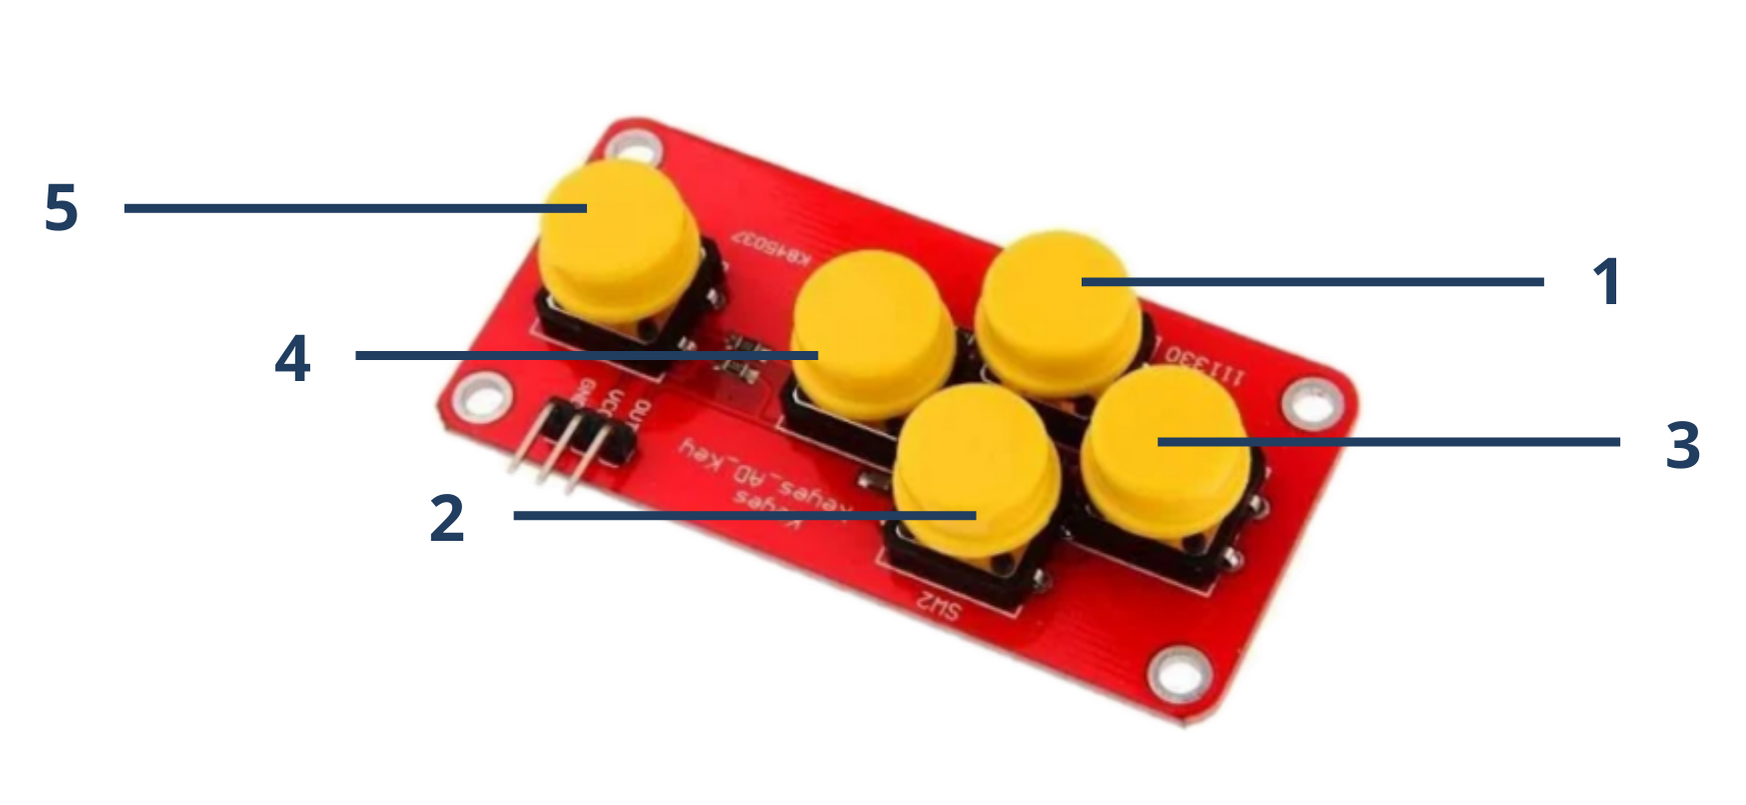
\includegraphics[width=0.6\textwidth]{figuras/eletronica/fotos_componentes/num_teclado.png}}
    \caption{Foto do teclado.} %Identificação do Botão  1- CIMA, 2- BAIXO, 3- DIREITA, 4- ESQUERDA, 5- SELECIONE}
    \label{fig:botoes_identificados}
\end{figure}

O botão 1 tem que subir as telas da interface, o botão 2 descer as telas, o botão 3 muda em telas específicas para direita, o botão 4 para esquerda e o botão 5 é realiza a seleção/\textit{enter} da interface, confirmando e selecionando alguma opção. 

\subsection{Teste do Módulo de Medição}

Para o teste do módulo de medição primeiro é necessário checagem individual de cada sensor nele contido. Onde será avaliado se o sensor não apresenta defeito ao atender os resultados esperados.

Concluída a validação individual de cada sensor será realizado testes específicos de integração com componentes da central de controle em que são conectados, conforme descrito na arquitetura do sistema eletrônico na seção \ref{sec:arq_eletronica}.

\subparagraph*{$\bullet$ Sensor de Temperatura e Umidade: HTU21D} \hfill

% A primeira etapa consiste em testar a conexão entre o sensor e a central de controle, utilizando para isso um programa básico de detecção para o protocolo I$^2$C. 

Para o sensor HTU21D está sendo considerado que o teste de conexão com a central de controle foi realizada na etapa anterior, nos testes da central de controle. Assumindo que a aquisição dos dados por I$^2$C está funciona pode-se prosseguir para o primeiro teste. 

O primeiro teste consiste em verificar os valores que estão sendo medidos de temperatura e umidade relativa para calibração a valores padrão em um ambiente controlado. Pra melhor calibração é recomendado o uso de um equipamento de terceiro com calibração própria que realize medições de temperatura e umidade com mesma ou maior precisão que o sensor utilizado. Também é necessário o uso de um ambiente controlado que pode variar entre 5 $ ^\circ$C e 55 $^\circ$C.

Utilizando um programa simples é requisitado os valores de temperatura e da umidade relativa em um período de 5 minutos, onde os dados são armazenados para análise e calibração. Segundo o fabricante o sensor vem calibrado de fábrica portanto as compensações feitas por esse teste são para atingir uma acurácia específica. Sendo observado se existe um erro menor que 5\% comparado a medida do equipamento externo usado na calibração (caso esteja sendo utilizado).

Com a curva de calibração traçada para o ambiente controlado, está é inserida no algoritmo de processamento para um segundo teste. Esse teste consiste na validação da calibração em situações controladas de funcionamento normal da máquina para chegar a acurácia do modelo levantado. 


\subparagraph*{$\bullet$ Chave: Micro \textit{Switch} KW10-B} \hfill

Para as chaves primeiro é realizado um teste de continuidade entre os terminais 1 e 2 utilizando um multímetro para verificar se existe alguma chave com defeito. Nesse teste é crucial garantir que a chave está sendo clicada corretamente para não gerar falso-positivo quanto a existência de continuidade. 

Em seguida, é realizado um segundo teste que verifica se a central de controle está conseguindo detectar a abertura e fechamento de cada chave. Semelhante a testes realizados na central de controle é necessário rodar um programa básico de testes na \textit{Raspberry Pi} 4 para que seja possível observar cada chave conectada ao microcontrolador 2. 

Primeiro deve se fazer o teste com todos as chaves pressionadas (portas fechadas caso já foram instaladas). Em seguida, repita o procedimento soltando as chaves (ou portas abertas caso foram instaladas). Caso ocorra falha na detecção em algum dos componentes primeiro verifique a conexão da chave com a respectiva PCI. Esse procedimento inclui tanto a verificação da conexão entre a PCI e a chave quanto do cabo utilizado, verificando se o mesmo não apresenta algum rompimento ao utilizar um multímetro para averiguar a continuidade do par de terminais. 

Repita os dois testes e, caso o erro não foi solucionado e a chave não apresentou defeito no teste, pode-se concluir defeito ou do C.I. MUX/DEMUX relacionado a chave com problemas ou no microcontrolador. Para solução desse problema primeiro troque o C.I. MUX/DEMUX relacionado a chave defeituosa, usando como guia em qual remover o esquemático 3 na Fig. \ref{fig:esquematico_3}. Se não o microcontrolador da PCI, sendo necessário o teste da conexão com a \textit{Raspberry Pi} 4 e descrito na seção \ref{sec:teste_cc}.

\subparagraph*{$\bullet$ Sensor Fotoelétrico} \hfill

O primeiro teste realizado com os sensores de barreira é a verificação da saída do comparador na PCI de cada um. Sendo assim, é utilizado um teste de bancada que contém uma plataforma que simula as 5 diferentes distâncias entre o emissor (\textbf{IR333C}) e receptor (\textbf{PT333-3B}) encontradas internamente no dispositivo (10,45 mm para contêiner, 66,19 mm para o funil, 55,15 mm reservatório de copos, 145,28 mm para local de detecção do copo abaixo da câmera e 103,9 mm para porta frontal ou traseira). A verificação da saída do comparador é realizada em um osciloscópio para observar se atende as especificações desenvolvidas. 

No procedimento de testes é colocado um obstáculo que simula o volume de um comprimido e de um copo para respectivas distâncias onde esses objetos passariam no dispositivo, sendo repetido vezes suficientes para ter confiança do funcionamento para todos os casos. Caso seja detectado alguma saída errada e não está relacionado a conexão entre a PCI e os fotosensores pode-se concluir que o comparador LM398, sendo necessário sua troca por um novo. 

Passando o teste de bancada pode-se prosseguir com a instalação, seguindo o procedimento na seção \ref{sec:construcao_modulo_medicao}. Concluída a instalação na estrutura e conexão com a PCI com respectivo microcontrolador é realizado o teste de funcionamento com a central de controle. Esse teste se utiliza um código simples que realiza verifica a saída de cada sensor de barreira por um período de 10 segundos, trocando por esse intervalo para o próximo até concluir os 30 sensores. Durante os 10 segundos se alterna a colocação de um obstáculo para observar se a central de controle está recebendo a resposta apropriada. Caso ocorra algum erro na detecção de algum sensor de barreira é realizado o mesmo procedimento descrito anteriormente para as chaves KW10-B. Onde é verificado a conexões, os cabos, o C.I. MUX/DEMUX e o microcontrolador, trocando na conclusão que é uma peça defeituosa.


\subparagraph*{$\bullet$ Sensor de Biometria: DY50} \hfill

Considerando que o teste de conexão com a central de controle foi realizada com sucesso é necessário a realização de testes para verificar as funcionalidades básicas e parâmetros de confiabilidade do sensor de biometria DY50. Nos testes inicias consistem em rodar um programa simples que inclua as bibliotecas do fabricante, conforme descrito no \textit{datasheet}, para averiguar funcionalidades básicas de registro, detecção e remoção de impressões digitais. 

Para propósitos de teste inicial é recomendado testar com as 10 digitais da mão de um único usuário. Primeiro se registra as 10 digitais, e, após a validação do programas que todas foram corretamente registradas, realizar o teste de detecção. Nesse teste é colocado cada dedo e verificado no terminal se o programa está conseguindo detectar o dedo que foi registrado, repetindo o processo por pelo menos 10 vezes para cada dedo. 

Por fim, é realizado o teste de remoção para averiguar se, após deletar uma digital, não existe a detecção dela pelo sistema. Primeiro é requisitado a remoção da digital no banco de dados, com ID especificado durante o registro, e é realizado 10 tentativas de detecção daquele dedo pelo sensor de biometria. Caso a detecção falhe, conforme esperado, pode-se concluir que o sensor está funcionando de forma correta.

Na segunda bateria de teste é realizado a verificação de confiabilidade do registro da digital pelo sensor. Esse processo busca analisar o valor de confiança mínima para o sensor utilizado não considerar situações falso-positivas. O fabricante não descreve uma metodologia específica porém realizamos esse teste com o registro das digitais de pelo menos 5 pessoas distintas. Sendo assim, são realizados testes monitorando o valor de confiança que a digital tem para cada digital, repetindo o processo em vários ciclos até concluir um valor ótimo para aplicação no produto.

\subparagraph*{$\bullet$ Sensor de Leitura RFID: PN532} \hfill

Para o sensor PN532, após a averiguação de correta conexão usando protocolo I$^2$S com a central de controle, conforme descrito no plano de testes dela, será verificado o funcionamento da leitura e escrita para as etiquetas dos copos de medicamento. Para esse teste é utilizado um programa simples que roda o processo de detecção e registro de informação na etiquetas RFID do copo. 

O procedimento consiste em colocar o copo na posição logo abaixo do funil, local onde o copo sai do reservatório de copos e o sensor RFID foi posicionado, verificar foi possível realizar a escrita de um ID na etiqueta. Caso tenha um celular/dispositivo compatível retire o copo da posição e realize a leitura da etiqueta, verificando se os dados que deveriam ser armazenados condizem com o lido. Em seguida se repete o mesmo procedimento porém para realizar a leitura da informação armazenada na etiqueta e comparação com o que deveria ser o resultado, conforme armazenado previamente no banco de dados. Esse procedimento se repete para todos os copos suportados pelo dispositivo. 


\subparagraph*{$\bullet$ Câmera: OV5647} \hfill

Para o teste da Câmera OV5647 utilizamos o mesmo programa descrito no teste da central de controle, que realiza a detecção da conexão e tira uma foto. O teste consiste em verificar exposição, cores, brilho, zoom e o funcionamento junto com o flash no local onde ele é utilizado. 

Sendo assim, é colocado um copo com alguns comprimidos registrados no banco de dados do sistema abaixo da câmera, simulando onde estaria o copo durante o uso desse sensor. Em seguida, rodamos um programa simples que detecta a câmera e tira uma foto com flash. Analisando a foto tirada faça ajustes finos do zoom e intensidade do flash caso necessário. Por fim, realize uma série de fotos com a câmera calibrada para verificar se existe algum problema no sensor. 
As fotos são utilizadas em outro código relacionado ao processamento de imagens, conforme descrito anteriormente na solução. Caso não seja possível detectar os comprimidos de teste reveja a calibração do zoom, flash, exposição e cores. Repita o processo e se persistir o problema realize a troca da câmera. 

\subsection{Teste do Módulo de Acionamento dos Atuadores}

Os testes realizados para o módulo de acionamento dos atuadores tem objetivo de verificar o funcionamento dos componentes utilizados atendem simulações de controle ou cálculos, observando por um ponto de vista da parte elétrica com enfase no controle. A explicação por um ponto de vista estritamente elétrico da alimentação dos motores como de características elétricas são descritas no plano de teste da solução de energia, seção \ref{sec:plano_teste_energia}.

Para cada atuador são realizadas 3 fases de testes sendo: Teste Inicial, Teste Parcialmente Integrado e Teste Completamente Integrado seguindo o seguinte procedimento:

% \begin{itemize}
% \item[]
% \begin{itemize}

\subparagraph*{} $\bullet$ \textbf{Teste Inicial:}
    
Nessa fase cada componente relacionado ao funcionamento dos atuadores são testados por um ponto de visto elétrico. Como testes de comportamento elétrico ao interligar \textit{driver} e atuador e de operação do respectivo microcontrolador que realizado a distribuição do sinal de controle com os atuadores. Sendo realizado para validar a correta funcionalidade dos componentes comparado ao que era esperado.
    
\newpage
    
\subparagraph*{} $\bullet$ \textbf{Teste Parcialmente Integrado:} \hfill 

Nessa fase de teste alguns componentes elétricos são interligados para mostrar que essa integração vai ter mínimo impacto no comportamento dos atuadores, sendo analisado principalmente o erro. Isso é realizado com uma integração simples do atuador e respectivo \textit{driver} com a central de controle. Onde é executado vários testes simples do controle e realizado medições de várias tolerâncias que impactam como o projeto. Essa etapa é crucial para realizar calibração e implementar ajustes antes de fixação dos atuadores no dispositivo protótipo.
    
\subparagraph*{} $\bullet$ \textbf{Teste Completamente Integrado:} \hfill

Nessa fase, os componentes mecânicos do dispositivo são integrados com os componentes elétricos previamente testados. Os principais pontos testados e analisado são as tolerâncias e se o funcionamento correto dos atuadores sob condições normais de carga atendem e superam as especificações projetadas. 

% Ademais, alguns problemas que podem acontecer na integração como potência, geração de calor, vibração, peso e ajustes fino em parâmetros de controle são resolvidos durante essa etapa.

% \end{itemize}
% \end{itemize}

\subparagraph*{$\bullet$ \textit{Driver} Motor de Passo: A4988} \hfill

\subparagraph*{} $-$ Teste inicial:\label{sec:teste_inicial}

O primeiro teste consiste em realizar medições da tensão elétrica de alimentação e sinal de controle entre motor de passo, \textit{driver} e circuito integrado com microcontrolador.  O equipamento necessário para essa medição é um multímetro. Nesse teste temos o seguinte critério a se satisfazer:

\begin{itemize}
    \item $V_\text{alimentação}$ = 12 V
    \item $V_\text{controle}$ = 5 V 
\end{itemize}

O procedimento consiste em testar cada terminal e GND para verificar a tensão fornecida pela fonte de alimentação para o \textit{driver} A4988 está correto. Repetindo para os 5 utilizados.

Completando o primeiro teste é garantido que os componentes usados atendem as especificações técnicas elétricas e não estão com defeito. Assim como as perdas no cabo não são bem especificadas.

O segundo teste é para testar a operação do circuito integrado com microcontrolador. Sendo verificado a resposta dos vários sinais de controle do \textit{driver} para uma rotina normal de operação. As especificações analisadas são as seguintes:

\begin{enumerate}
    \item Geração do sinal lógico para entrada \textit{STEP}
    \item Nível lógico para as outras 6 entradas (MS1, MS2, MS3, DIR, ENABLE, RESET).
    \item Modos de operação:
    \begin{enumerate}
        \item Modo de espera
        \item Operação na velocidade máxima
        \item Operação na metade da velocidade
        \item Operação de parada
        \item Modo de inicialização
        \item Cenário com falha na alimentação
    \end{enumerate}
\end{enumerate}

No procedimento de teste é utilizado um programa básico rodando na Raspberry Pi 4 que simula o controle dos motores de passo. Para medição dos terminais é utilizado o osciloscópio para verificar se os sinais gerados estão condizentes com o desenvolvido para o projeto. 

O critério para aprovação é verificar se os sinais enviados estão dentro dos parâmetros operacionais do controle e se podem pode ser interpretado pelo \textit{driver} sem erros.

\subparagraph*{} $-$ Teste Parcialmente Integrado:\label{sec:teste_parc_int}

O primeiro teste verifica se os motores de passo estão sendo controlados corretamente ao conectar o \textit{driver} A4988 com a central de controle. Para avaliação inicial do controle não é aplicado nenhuma carga e são realizadas medições de temperatura e corrente. Esse teste segue as seguintes especificações:

\begin{enumerate}
    \item Habilitar e desabilitar cada motor
    \item Rotação do motor
    \begin{enumerate}
        \item Girar na rotação horária (um passo)
        \item Girar na rotação anti-horária (um passo)
        \item \textit{Reset} do \textit{driver}
    \end{enumerate}
    \item Operação normal do sinal lógico para terminal \textit{STEP}
    \item Medição de temperatura
\end{enumerate}

O procedimento consiste em conectar tanto \textit{driver} (já ligado com o motor) na respectiva PCI PIC16 4 que contém o microcontrolador quanto a alimentação para iniciar os testes. Em seguida, é inicializado na Raspberry Pi 4 uma rotina de controle simples para realizar medições para verificar as especificações descritas acima. Os sinais são medidos usando um osciloscópio verificando os sinais de entrada e saída do \textit{driver} para mostrar o sinal de controle gerado pelo microcontrolador e respectiva resposta enviada para os motores de passo.  Para validar quão robusto é essa integração será variado o fator de ciclo (\textit{duty cycle}) do sinal lógico de controle, observando se a velocidade de giro varia nas proporções corretas. 

Os critérios de aprovação desse teste são:
\begin{itemize}
    \item Rotação dos motores nas direções corretas;
    \item Operação correta na condição sem carga;
    \item Sinais recebidos pela conexão entre o \textit{driver} e a controle estão corretos;
    \item Rotação do motor respondendo corretamente á variação do fator de ciclo. 
\end{itemize}

\subparagraph*{} $-$ Teste Completamente Integrado:\label{sec:teste_comp_int}

Nesse teste será avaliado a performance dos motores de passo quando conectados a estrutura do dispositivo, ou seja, montagem na posição correta e fixação do fuso. Sendo assim, é avaliado se existe a necessidade de modificações adicionais nos parâmetros de controle para a condição de carga adicionada após integração.

O procedimento consiste em realizar a montagem dos 5 motores de passo, 5 \textit{drivers} A4988 e conexão com a PCI da central de controle, especificada como PIC16 4. Em seguida, é executado um programa teste do controle na Raspberry Pi 4 para esse motores. Sendo realizados medição da velocidade de rotação para vários períodos de tempo diferentes. Também é avaliado se o tempo de resposta dos motores após ser enviado um comando está rápido o suficiente para o bom funcionamento do dispositivo. 

Os critérios de aprovação são:

\begin{itemize}
    \item Execução dos comandos de controle pelos motores dentro das tolerâncias para queda de um medicamento do contêiner;
    \item Carga elétrica consumida pelos motores durante rotação normal não afeta o funcionamento de outros dispositivos;
    \item Velocidade de operação adequada dos sinais recebidos da central de controle para o \textit{driver}.
\end{itemize}


\subparagraph*{$\bullet$ \textit{Driver} Motor DC: L298} \hfill

\subparagraph*{} $-$ Teste inicial:

Para a fase de teste inicial para \textit{driver} L298 para motor DC segue o mesmo procedimento e critérios de avaliação descritos para o motor de passo, descrito anteriormente em \ref{sec:teste_inicial}. Sendo que a única alteração é que, para avaliação da operação do microcontrolador, a especificação analisada é a geração do sinal PWM ao invés de pulsos elétricos. 

\subparagraph*{} $-$ Teste Parcialmente Integrado:

Para a fase de teste parcialmente integrado para \textit{driver} L298 do motor DC conectado a central de controle segue o mesmo procedimento descritos para o motor de passo, descrito anteriormente em \ref{sec:teste_parc_int}. No caso do motor DC serão avaliados as seguintes especificações: 

\begin{itemize}
    \item Rotação horária (Velocidade máxima)
    \item Rotação horária (Metade da Velocidade)
    \item Rotação anti-horária  (Velocidade máxima)
    \item Rotação anti-horária  (Metade da Velocidade)
    \item Freio (Curto do motor)
    \item Freio (Desabilitar o motor)
    \item Modo de operação correto para os sinais PWM
\end{itemize}

\subparagraph*{} $-$ Teste Completamente Integrado:

Para teste final é segue o mesmo procedimento de avaliando descrito para o motor de passo, em \ref{sec:teste_comp_int}. No caso do motor DC devemos integra-lo a esteiro do dispositivo. As especificações avaliadas para essa integração são as seguintes:

\begin{itemize}
    \item Tempo de inicio para movimentação da esteira
    \item Velocidade de rotação para vários períodos diferentes, avaliando consumo elétrico e performance
    \item Tempo para parada total da esteira com o freio
    \item Resposta ao controle condizente com a  projetada
\end{itemize}

O critério de aprovação será os tempos de resposta, velocidade e rotina de controle estão dentro das tolerâncias para funcionamento correto da esteira.

\subparagraph*{$\bullet$ \textit{Driver} Solenoides e Atuador linear: IRF520N} \hfill

\subparagraph*{} $-$ Teste inicial:

Para a fase de teste inicial do \textit{driver} IRF520N segue o mesmo procedimento e critérios de avaliação descritos para o motor de passo, descrito anteriormente em \ref{sec:teste_inicial}. Sendo que a única alteração é que, para avaliação da operação do microcontrolador, são observadas se o sinal lógico de ativação do solenoide ou atuador estão corretos.

\subparagraph*{} $-$ Teste Parcialmente Integrado:

Para a fase de teste parcialmente integrado do \textit{driver} IRF520N conectado a central de controle segue o mesmo procedimento descritos para o motor de passo, descrito anteriormente em \ref{sec:teste_parc_int}. No caso desse \textit{driver} serão avaliados as seguintes especificações: 

\begin{itemize}
    \item Sinal de controle enviado condiz com a resposta dos solenoides
    \item Tempo para ativação dos solenoides
    \item Tempo para desativação dos solenoides
    \item Consumo de potência condizente sob condição sem carga
\end{itemize}

\subparagraph*{} $-$ Teste Completamente Integrado:

Para teste final é segue o mesmo procedimento de avaliando descrito para o motor de passo, em \ref{sec:teste_comp_int}. No caso dos solenoides são instalados 25 para os contêineres, e 7 para as portas (1 frontal e 6 superiores) e para o atuador linear temos a instalação na base do reservatório de copo. As especificações avaliadas para essa integração são as seguintes:

\begin{itemize}
    \item Tempo de resposta para abertura e fechamento das solenoides dentro da tolerância
    \item Tempo de resposta do atuador linear está dentro da tolerância
    \item Velocidade de abertura e fechamento das solenoides dentro das tolerâncias
    \item Velocidade de acionamento e fechamento do atuador linear dentro das tolerâncias 
    \item Rotina de controle condizente com a projetada
\end{itemize}

O critério de aprovação será os tempos de resposta, velocidade e rotina de controle estão dentro das tolerâncias para funcionamento correto dos solenoides quanto do atuador linear.

%\section{Teste de Integração}

%\ref{fig:PCB_barreira}
%\ref{fig:PCB_central}
%\ref{fig:PCB_micro1}
%\ref{fig:PCB_micro2}
%\ref{fig:PCB_micro3}
%\ref{fig:PCB_micro4}